\documentclass[a4paper]{article}

\usepackage[english]{babel}
\usepackage[utf8]{inputenc}
\usepackage{url}
\usepackage{amsmath}
\usepackage{graphicx}
\usepackage{float}
\usepackage{wrapfig}
\usepackage{caption}
\usepackage[colorinlistoftodos]{todonotes}
\usepackage{verbatim} % for use of multi-line comments (using \begin{comment}...\end{comment}).
\usepackage[T1]{fontenc}
\usepackage{listings}
\usepackage{cleveref}
\crefname{figure}{figure}{figures}
\lstset{basicstyle=\ttfamily\small}
\setlength{\parskip}{0.8em}
\addtolength{\topmargin}{-.5in}
\addtolength{\oddsidemargin}{-.5in}
\addtolength{\evensidemargin}{-.5in}
\addtolength{\textwidth}{1.0in}
\addtolength{\textheight}{0.7in}

\definecolor{mygreen}{rgb}{0,0.6,0}
\definecolor{mygray}{rgb}{0.5,0.5,0.5}
\definecolor{mymauve}{rgb}{0.58,0,0.82}
\lstset{ %
  backgroundcolor=\color{white},   % choose the background color
  basicstyle=\footnotesize,        % size of fonts used for the code
  breaklines=true,                 % automatic line breaking only at whitespace
  commentstyle=\color{mygreen},    % comment style
  escapeinside={\%*}{*)},          % if you want to add LaTeX within your code
  keywordstyle=\color{blue},       % keyword style
  stringstyle=\color{mymauve},     % string literal style
}



\title{GreenMirror: A Visualization Framework for State-Transition Models}
\author{Karim El Assal \\ s1097539}
\date{\today}



\begin{document}




\maketitle

\begin{abstract}
State-transition models are often used to analyse the discrete dynamic behaviour of systems, although analysis may prove to be tedious when a system has a huge amount of possible states. A framework using the Java programming language and the JavaFX library is being developed to provide a different approach. Continuing previous work, the next step has now been made in the development, resulting in a version that can visualize a system's states and animate transitions that result from a list of state-transitions. The user can define complex state-transition models during runtime which will be visualized according to the state-transitions the user also provides during runtime. The framework has been specifically designed to support future development by being modular, extendible and maintainable.

\end{abstract}

\newpage
\tableofcontents

\newpage




%----------------------------------------------------------------------------------------
%------------------------------------------------
%------------------------ Introduction
%-------------
%------
\section{Introduction}

%--------------------------------
%----------------
%-------- Background
%----
%--
\subsection{Background}\label{subsec:background}
State-transition models describe the discrete dynamic behaviour of a system. Such a model defines how the state of a system changes as the result of a trigger, and following its set of rules. In the field of computer science, these models are used for system verification and they can be analysed in several ways. One often used way is by means of a \emph{state space generation} tool such as GROOVE (see \cite{rensink2004}).

The state spaces generated by such tools can become huge, complex and difficult to analyse. The research group Formal Methods and Tools\footnote{\url{http://fmt.cs.utwente.nl/}} of the University of Twente has set out to develop a framework based on the Java programming language and the JavaFX library that enables researchers to analyse state-transition models using a different approach. The idea is to visualize the system state and animate the state-transitions based on a state-transition model with the goal of gaining a better understanding of the model and its flaws.

The first step in the development of this framework has been made by Alex Aalbertsberg (see \cite{aalbertsberg2015}). This report describes which further progress has been made since then to reach the current version that has been named \emph{GreenMirror}. Although the project is still in its infancy, hopefully these contributions will eventually lead to better state-transition model research.


%--------------------------------
%----------------
%-------- Glossary
%----
%--
\subsection{Glossary}\label{subsec:glossary}
\begin{description}
\item[The application] This refers to the GreenMirror application as used by the user to reach the goal as intended by the developer. It is a compiled version of the source code that is the GreenMirror framework.
\item[The framework] This refers to the application in development and specifically its source code.
\item[GreenMirror] The name of this project. It does not have a profound meaning, it is chosen to have a short designation to indicate that this project is meant in certain contexts.
\item[JavaFX transition] The animation of a JavaFX node property from one value to another.
\item[The (researched/user-defined) model] The model that the user wants to visualize and research using the GreenMirror application.
\item[State] The state of a user-defined model.
\item[State-transition] A transition from one state of the user-defined model to another. In the visualizer, this can contain multiple JavaFX transitions.
\item[State-transition model] A model that describes how a system transitions from one state to another.
\item[Trace] A sequence of state-transitions.
\item[User] The user is the researcher that uses the framework to visualize certain models (see \cref{subsec:stakeholders}).
\item[Visualizer] The component of the GreenMirror application that actually visualizes the states and the state-transitions.
\end{description}

%--------------------------------
%----------------
%-------- Stakeholders
%----
%--
\subsection{Stakeholders}
\label{subsec:stakeholders}
It is assumed that any stakeholder knows what he is doing when interacting with the system in the sense that the stakeholder knows about the context and the tools he is using. There are three ways of interaction, so the groups of stakeholders are divided as such.
\begin{description}
\item[\textbf{The user}] The end-user, or "user" for short, is the stakeholder that uses the application for its main purpose: visualizing models. The "user" can also be renamed "the visualization builder", but in this report the term "user" will be retained. The user is expected to have a basic understanding of programming in general and specifically of the Java language.
\item[\textbf{The state space tool owner}] Researchers might want to connect their own state space tool to the GreenMirror framework. The development of a suitable interface for this is taken into account in the design of the framework. Any person that writes a new extension to connect his state space tool to the GreenMirror framework is called a "state space tool owner", or "tool owner" for short, and will be considered in the design and development phases.
\item[\textbf{The developer}] The GreenMirror framework is intended to be extended and otherwise improved over time. The developers that will do so are also seen as a relatively small group of stakeholders. To extend and improve the framework developers will need an in-depth understanding of the framework, contrary to tool owners who only need to understand the interface between their tool and the framework. Hence, large part of this report is written for developers.
\end{description}









%----------------------------------------------------------------------------------------
%------------------------------------------------
%------------------------ Project definition
%-------------
%------
\section{Project definition}\label{sec:projectdefinition}
The main goal of this project is to make it possible for researchers to visually analyse the temporal behaviour of state-transition models. These models are already defined and have already been visualized in a different way in state space tools, as described in {\cref{subsec:background}}. The framework should be easily extendible and modifiable, so it can be improved in the future. Several requirements are described in the following subsections to properly define the requisites that will be used in the design and development phases. All requirements are \emph{MoSCoW} formulated.

%--------------------------------
%----------------
%-------- Architectural requirements
%----
%--
\subsection{Architectural requirements}
In the architectural requirements of the framework, the developer is the main stakeholder since he has most to gain from a well-defined software system. These requirements are fairly general and vague, but have to be stated nevertheless.
\begin{description}
\item{\textbf{Extendibility}} The framework must be easily extendible. Future research might require new functionalities, so a developer or tool owner must be able to extend in stead of heavily modify the source code.
\item{\textbf{Maintainability}} A developer must have little to no effort in understanding the source code when improvements or extensions are developed. Programmed structures and patterns must be easily recognizable and well documented.
\end{description}
From these requirements, one could extract the implicit requirement of modularity. Although it is not defined as a fixed requirement, it will be taken into account.

%--------------------------------
%----------------
%-------- Functional requirements
%----
%--
\subsection{Functional requirements}\label{functionalrequirements}
All functional requirements relate to the application, seeing as the application contains functionality and the framework does not. Therefore, the user is the main stakeholder in these requirements. In general, the application has to be \emph{flexible}. The user is assumed to be a researcher, which implies that the user wants to have as much freedom as possible in deciding what the application does, how it works and what it gives as output. This requirement is the basis for all following requirements, which are mostly described in the order of usage by the user.
\begin{itemize}
\item \textbf{The application must become aware of the researched model} and how to visualize it. This process is divided into several parts.
	\begin{itemize}
    \item The application must become aware of the initial nodes and relations the researched model is composed of.
    \item The application must become aware of how these initial nodes and relations should be visualized.
    \item The application must become aware of how state-transitions should be visualized.
	\end{itemize}
\item \textbf{The application must become aware of the trace}. Executing this trace gives the user the opportunity to analyse the model's dynamic behaviour.
\item The application must \textbf{show the visualization to the user} generated from the user's specified model. As a basis for this requirement, the application must be able to visualize simple shapes (such as rectangles, circles, text and images), simple animations (such as moving, creating and removing nodes) and the placement of one node in a specific respect to another. See \cref{subsec:requirementsvalidation} for specifics.
\item The application should \textbf{provide a detailed log} about what it has done. This helps in debugging and improving the application and in analysing the researched model.
\item As a result of the user's interactions, the application should be able to \textbf{move back and forth between the transitions} given by the trace while consistently seeing the proper visualization and without errors or reduced performance. This way the user doesn't have to rerun the complete application on each examination of the model.
\end{itemize}

%--------------------------------
%----------------
%-------- Performance requirements
%----
%--
\subsection{Performance requirements}
The performance requirements also relate to the application and primarily concern the smooth and uninterrupted execution of visualizations.
\begin{itemize}
\item After the model has been loaded into GreenMirror, the visualizer should be able to \textbf{transition to a next or previous state without noticeable delay} caused by memory or processing problems.
\item While transitioning to a next or previous state, \textbf{the application should not crash} or terminate otherwise. This includes the assumption that the model has successfully been loaded into GreenMirror and all model logic has been deemed valid and without errors.
\end{itemize}

%--------------------------------
%----------------
%-------- Exclusions
%---- (Only added if sensible exclusions are encountered.)
%--
%\subsection{Exclusions}

%--------------------------------
%----------------
%-------- Possible extensions
%----
%--
\subsection{Possible extensions}\label{subsec:possibleextensions}
The scope of these contributions to the project are limited. Had it been larger, an extension that could have been implemented is the reverse of the current main goal of GreenMirror. In addition to visualizing a defined model, a model could be altered or even defined from scratch based on how the user interacts with the visualizer.
\\This can be explained by introducing the following, relatively simple scenario. Take a model where a state-transition results in the moving of a node from one location to another. With the proposed extension implemented, the user might now be able to drag a node in the visualizer from one location to another. Assuming both location boundaries have been properly defined, the application can recognize this as a state-transition. In this scenario the user can alter the trace, adding state-transitions before, in-between or after the transitions on the original trace.

There are of course many more visualization possibilities than simply moving a node. Amongst others, on which this report will elaborate more later, relations between nodes can be created and removed, nodes can change colour and size, new nodes can be added and existing nodes can be removed. This could also be implemented in an extension. Continuing and expanding on the previous scenario: in stead of the atomic interaction of dragging a node to another location, the user could record multiple changes in the visualizer resulting in one newly defined or previously defined, recognized state-transition. This might work fine solely for recognizing simple, previously defined state-transitions, but this still has considerable limitations in the creation of new state-transitions.

Another step that should be taken in the development of this extension to enable the user to create a model based on interactions with the visualizer, is the addition of the creation of model logic. In the GreenMirror application, a transition in the model could be defined as such: "if node A and node B both have a relation with node C, remove the relation between node A and node C and add a new relation between node A and node D". In this step of the development of this extension, a user should be able to create such logic based on his interactions with the visualizer. This can become complex very fast, but that is just an interesting challenge to accept in the future.

The next step is to make a two-way connection with other tools that enable or facilitate the research of state-transition models in different ways. When the connection is made between interactions with the visualizer and the creation of transition logic, this could be translated into a format that can be accepted by other tools. This way, the need is eliminated for researchers to rewrite their models into tool-specific formats when different tools are used.


%--------------------------------
%----------------
%-------- Requirements validation
%----
%--
\subsection{Requirements validation}\label{subsec:requirementsvalidation}
Several well-known test models have been defined to validate the functional and performance requirements. These models are not extremely complex, but they do depict the possibilities of the application and show that the requirements are met. All models described below validate the following functional requirements by simply showing the visualization. If one of these requirements is not met, the model could not have been visualized.
  \begin{itemize}
  \item The application must become aware of the researched model.
  \item The application must become aware of the trace.
  \item The application must show the visualization to the user.
  \end{itemize}
While viewing these models, sufficient data and information about what is happening should show in the log, as described by the requirement "show a detailed log". "Sufficient" in this context means in addition to all exceptions, everything that changes in the visualizer: adding and removing nodes and relations and changing visual properties of nodes.

\subsubsection{The ferryman}
This puzzle consists of four active objects: the wolf, the goat, the cabbage and the ferryman. In the initial state of the system, the first three objects are on the left bank of a river. The ferryman is moored to the same bank with his ferry. The goal is to transport the wolf, the goat and the cabbage to the right bank of the river. The following rules apply.
  \begin{enumerate}
  \item The ferryman can only bring one passenger at a time.
  \item If the wolf and the goat are together on either side of the river without the ferryman present, the wolf eats the goat.
  \item If the goat and the cabbage are together on either side of the river without the ferryman present, the goat eats the cabbage.
  \end{enumerate}
Possible transitions could be: \lstinline{load_wolf}, \lstinline{load_goat}, \lstinline{load_cabbage}, \lstinline{cross}, \lstinline{unload} and \lstinline{eat}. The application must at least be able to visualize 
  \begin{itemize}
  \item the banks of the river as two coloured rectangles;
  \item the wolf, the goat, the cabbage and the ferry as images;
  \item the loading of the passengers as their respective images moving from the bank they are on to the ferry;
  \item the crossing of the ferry with its (optional) passenger as their respective images moving to the other bank;
  \item the unloading of a passenger as its image moving from the ferry to the bank the ferry is moored to;
  \item the eating of the goat or the cabbage by letting the correct image disappear.
  \end{itemize}

\subsubsection{ConnectFour}
The game ConnectFour is such a well-known game that the rules will be left out of this report. The initial state of the system is an empty seven-by-six board and two players with differently coloured tokens. The application must at least be able to visualize
  \begin{itemize}
  \item the players' token colours; 
  \item the player whose turn it is and who is next, in textual form;
  \item the making of a move as a circular token falling through the specified column;
  \item the switching of the player whose turn it is.
  \end{itemize}

\subsubsection{The Dining Philosophers}
E.W. Dijkstra came up with the Dining Philosophers problem (see \cite{dijkstra1968}), which is often used to illustrate concurrency problems such as shared resources and deadlock scenarios. The problem scenario consists of a certain amount of forks and an equal amount of philosophers that sit around a table. Each philosopher has a plate of spaghetti in front of him and each pair of philosophers has a fork between them. The goal is to come up with a fair way for each philosopher to eat and don't die of starvation. The following constraints are in place.
\begin{enumerate}
\item Philosophers do only one of three things: think, be hungry or eat. They do not communicate with each other.
\item A philosopher needs two forks to eat and can only use the two forks on his immediate sides.
\item When a philosopher is thinking, he does not have forks and does not do anything at all.
\item When a philosopher gets hungry, he tries to obtain the two forks on his sides and will wait for their availability. He will not put down his first fork before he gets to eat.
\item After a philosopher is done eating, he releases the two forks.
\end{enumerate}
The forks represent shared resources in a concurrency problem. The constraints represent synchronization measures. A deadlock can, for example, occur when all philosophers get hungry at the same time and pick up the fork on their right.

The GreenMirror application should be able to handle this model. It should at least show
\begin{itemize}
\item philosophers around a circular table, as images of simple smiley faces as seen in \cite{magee1999};
\item the picking up and releasing of a fork, as the change of the philosopher's image;
\item and most importantly: the logic that comes with the state-transitions, bearing in mind that the actual order of state-transitions is determined by the trace.
\end{itemize}






%----------------------------------------------------------------------------------------
%------------------------------------------------
%------------------------ General design
%-------------
%------
\section{General design}\label{sec:generaldesign}
Nearly all design choices have been made bearing in mind that extendibility is one of the most important requirements. The first large, architectural choice that influences all other choices is the separation of the client and server roles. The client in this project is the component that interprets the user's model, whereas the server is the component that performs the actual visualization as a consequence of the changes in the model. With this separation, the two distinct components can be linked to other components or to other component versions in the future.

Tools such as GROOVE use \emph{nodes} and \emph{edges} to define their model. This terminology can not simply be copied, because the definition and usage of an edge is slightly different than the equivalent entity used in GreenMirror. GreenMirror uses \emph{nodes} and directional \emph{relations} to define the model. State-transitions consist of adding and removing nodes, altering the appearance of nodes and changing relations between nodes. \\
Node properties include a type, a name, labels and an appearance wrapper (more on this in \cref{subsec:implementationdetails}), all of which are optional. When the node is added to the model, it receives an internal identification number; "ID" for short. The user does not have to interact with this ID in any way. Nodes also store their relations with other nodes. \\
Relations are always directional, going from "node A" to "node B". All relations have a name, a placement, a rigidity and a temporary appearance for node A, of which the latter lasts for the duration of the relation. These properties are optional, although it is recommended to always specify a name. There are two kinds of relations: placement relations, indicating that node A has a placement relative to node B on the visualizer, and non-placement relations, where the placement is set to \lstinline{NONE}. The rigidity property can only be set for placement relations. When set to true it indicates that node A should follow when node B moves on the visualizer. If the rigidity is set to false, the placement is only calculated and applied when the relation is created: it won't be maintained when node B moves.

This might be overstating what has already been mentioned in \cref{subsec:glossary}, but in this project the term "node" is used two types of nodes: for a node in the model: a GreenMirror node; and a node of JavaFX: a (Java)FX node. When speaking simply of a node, a GreenMirror node is intended. In any other case, the words "JavaFX node" will be used. Solely using "FX" refers to the visual appearance of a GreenMirror node.

Different extendible parts of GreenMirror are loaded using the \lstinline{ServiceLoader} class, a dependency injector implementation of Java. This enables an easy and well-known way for adding new implementations and keeping an overview on which classes are implementations of which part.





%--------------------------------
%----------------
%-------- Package structure
%----
%--
\subsection{Package structure}
GreenMirror's package structure is fairly self-evident. Still, a short explanation per package is in place. The sub-packages that contain implementations of extendible features will be elaborated on in \cref{subsec:implementationdetails}. %See \cref{app:cd} for the class diagrams illustrating the relations between the classes.
\begin{description}
\item[\texttt{greenmirror}] is the main package containing classes shared by the client and server.
\item[\texttt{greenmirror.client}] contains all classes that pertain solely to the client.
\item[\texttt{greenmirror.client.modelinitializers}] contains all implemented model initializers that can be used by the client.
\item[\texttt{greenmirror.client.traceselectors}] contains all implemented trace selectors that can be used by the client.
\item[\texttt{greenmirror.commandlineoptionhandlers}] contains all command line option handlers, both for the client and server. The \lstinline{@ClientSide} and \lstinline{@ServerSide} annotations indicate where they are used.
\item[\texttt{greenmirror.commands}] contains all network commands that are sent from the client to the server or vice versa. The \lstinline{@ClientSide} and \lstinline{@ServerSide} annotations indicate where from where they are sent.
\item[\texttt{greenmirror.fxpropertywrappers}] contains all implemented wrappers for FX properties.
\item[\texttt{greenmirror.fxwrappers}] contains all implemented FX wrappers.
\item[\texttt{greenmirror.placements}] contains all implemented placements.
\item[\texttt{greenmirror.server}] contains all classes that pertain solely to the server.
\item[\texttt{greenmirror.server.playbackstates}] contains the playback states of the visualizer.
\item[\texttt{greenmirror.tests}] contains several unit and system tests to validate the workings of GreenMirror.
\end{description}


%--------------------------------
%----------------
%-------- General work-flow
%----
%--
\subsection{General work-flow}
\begin{figure}[ht]
  \centering
  \makebox[\textwidth][c]{
  	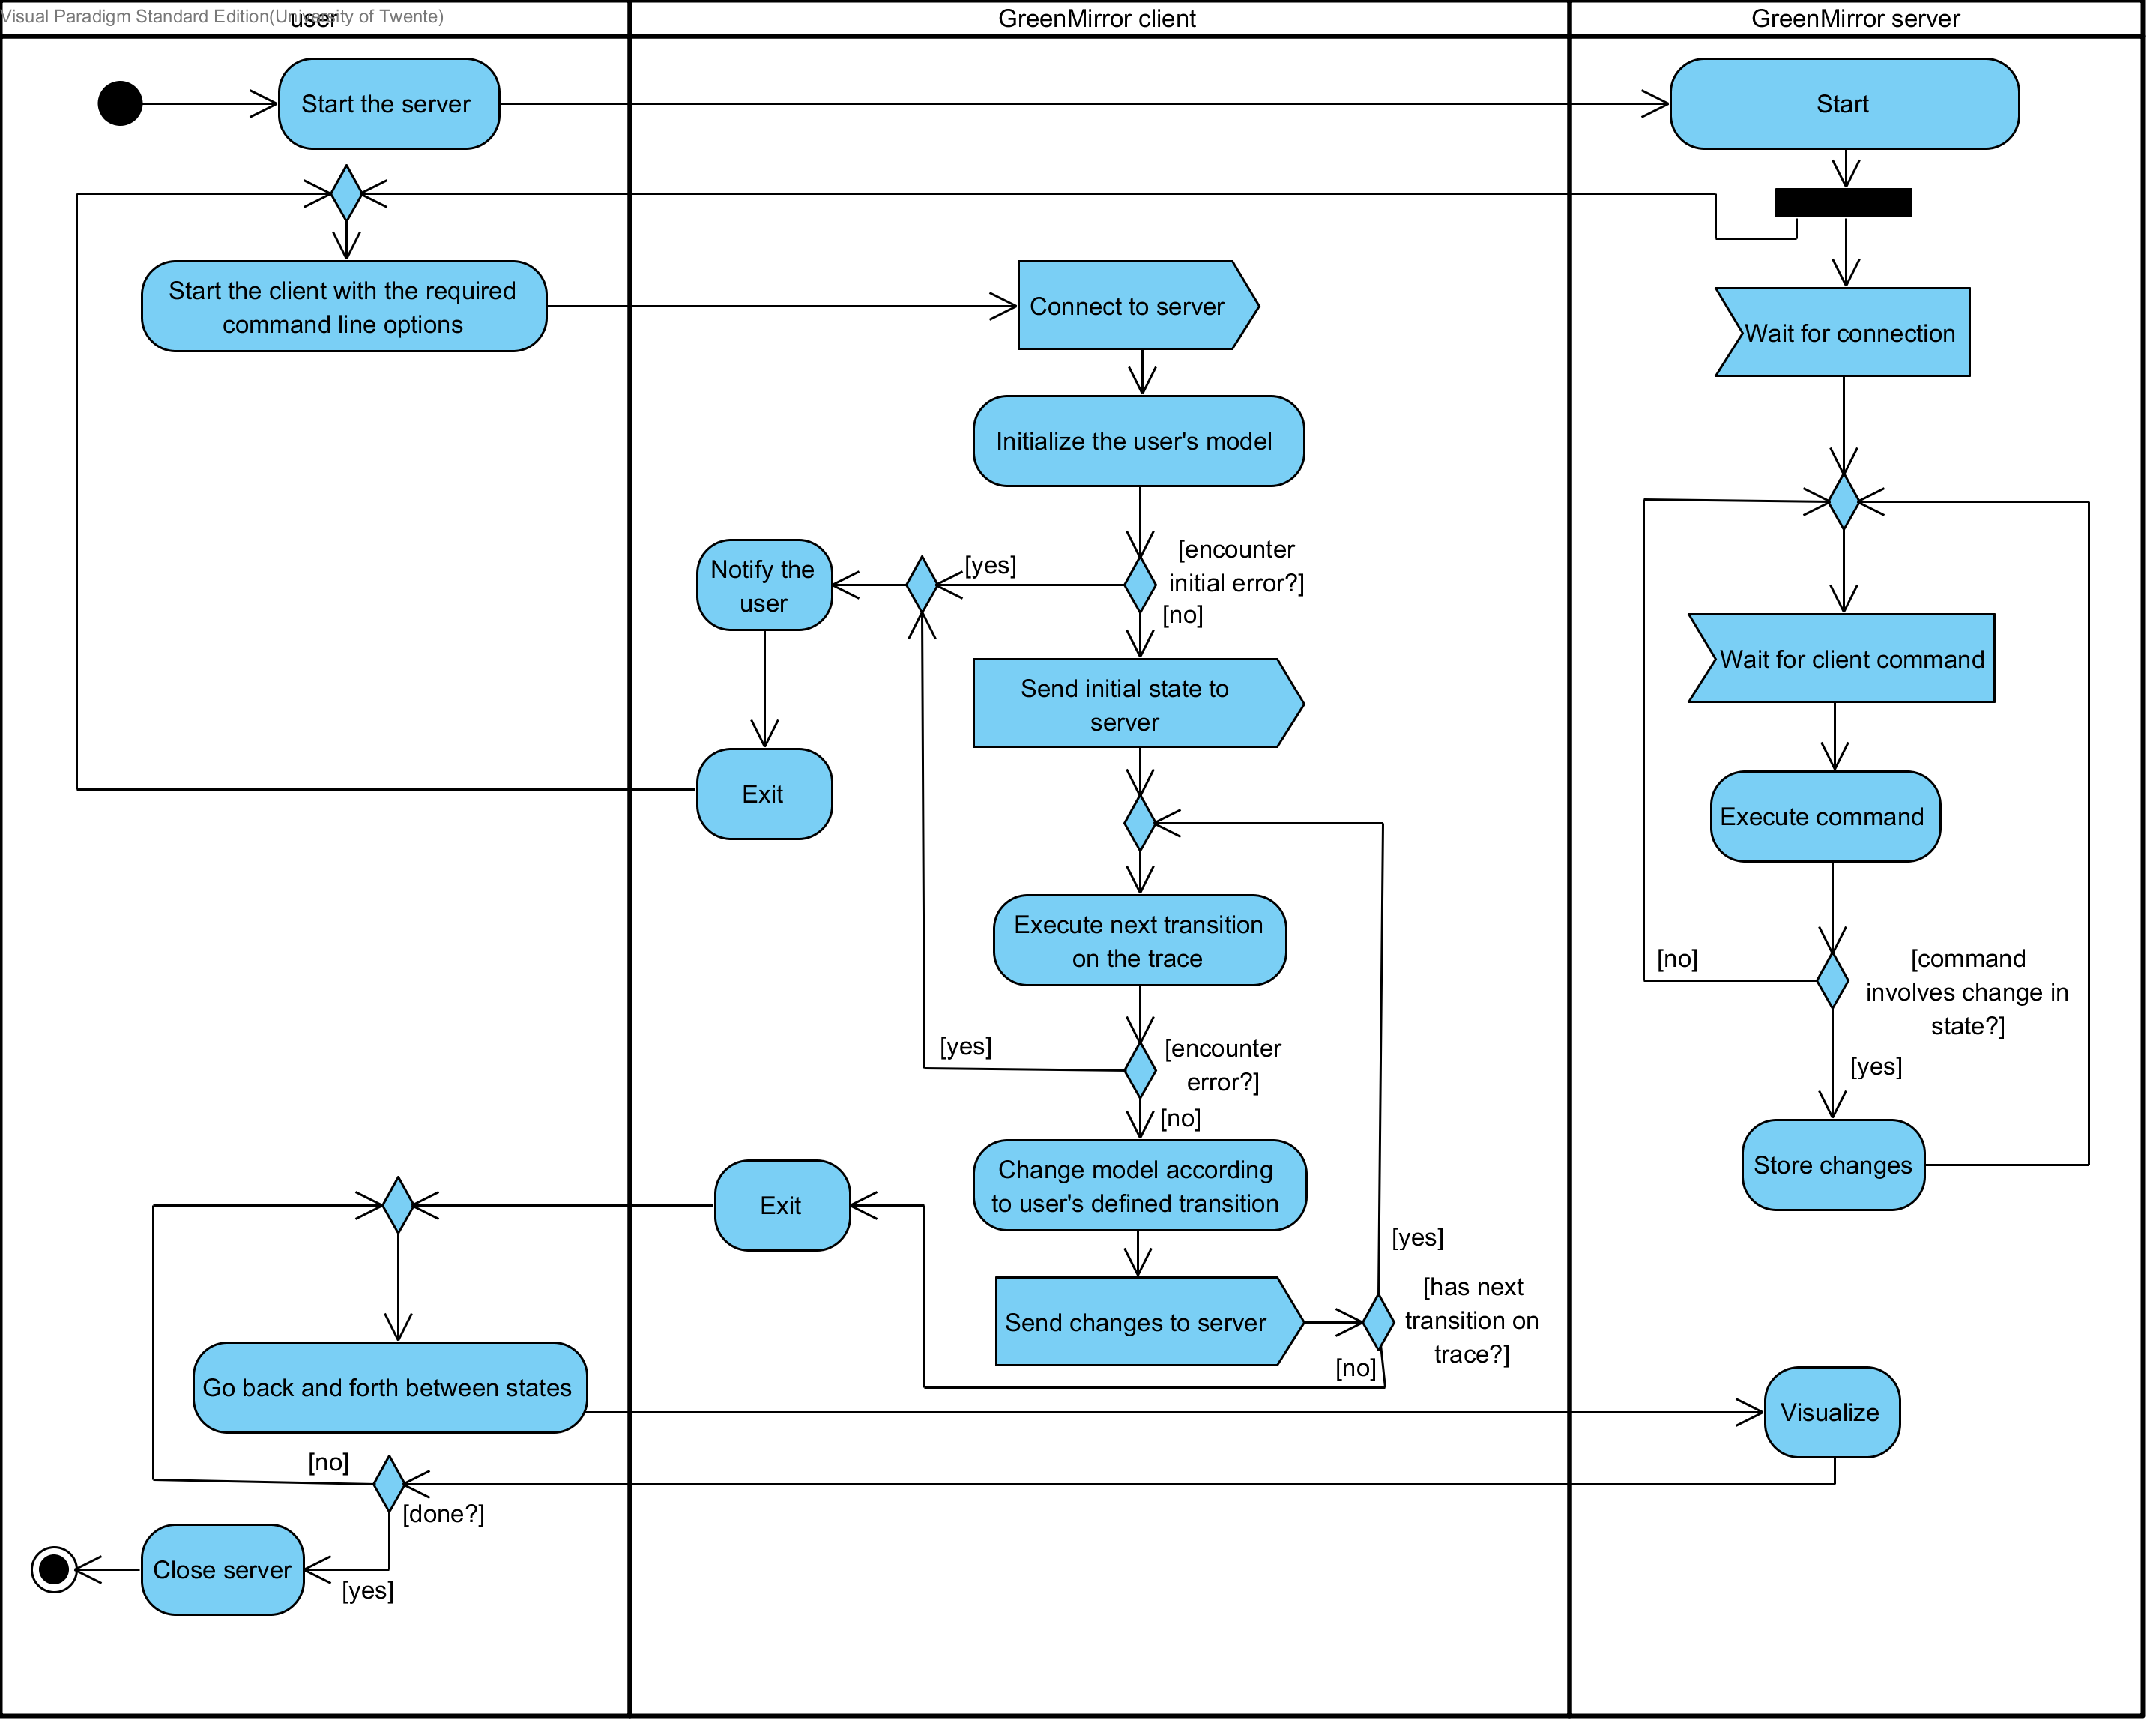
\includegraphics[width=1.0\textwidth]{diagrams/AD_generalworkflow}
  }
  \caption{Simplified activity diagram of the general work-flow (see \cref{app:ad} for a larger version)}
  \label{fig:ad_generalworkflow}
\end{figure}
The general work-flow of a typical execution of the application is illustrated in the simplified activity diagram of \cref{fig:ad_generalworkflow}. This is meant to be fairly general: the exact work-flow depends on the used model initializers, the used trace selector and the user's model. However, one note is worth mentioning. In the current design, the visualization can only start when the whole model has been interpreted by the client and has been sent to the server. This behaviour is meant to ensure top performance while transitioning through the states, but can be easily modified. 


%--------------------------------
%----------------
%-------- Detailed work-flow
%----
%--
\subsection{Detailed work-flow}\label{subsec:detailedworkflow}
Let's start at the beginning: starting up the client or server and parsing the command line options. GreenMirror uses the JOpt Simple library (see \cite{joptsimple}) to parse command line options in the same way options can be used with executables of *nix operating systems. Available command line options implement the \lstinline{CommandLineOptionHandler} interface. This contains everything needed to handle options: option and argument specification, processing order, argument validation and option processing. See \cref{fig:sd_generalstartup} (\cref{app:sd}) for the (simplified) sequence of these events. From the diagram can be seen that the options are all validated before they are processed. This prevents partial processing without having all required and valid options (for example: initializing the model without a valid server address).\\
The validating, parsing and processing of command line options, however, should not be understated. The complete set of the application's functions work as a direct consequence of the processing of these options. For example: the handler for the \lstinline{--host} option handles establishing the connection to the server and the handler for the \lstinline{--trace} option executes the trace. This results in the fact that new functionalities that should be executed during start-up can be easily added by implementing and adding new option handlers.

Now let's get into a little more detail about the specific command line option handlers of the client. From here on out, the assumption is made that all required options are passed (\lstinline{--host}, \lstinline{--model} and \lstinline{--trace}) and that their arguments are valid. If that would not be the case, GreenMirror would already have observed this and notified the user before terminating, as is described in the previous paragraph.

\begin{wrapfigure}{r}{0.38\textwidth}\vspace{-20pt}
  \begin{center}
    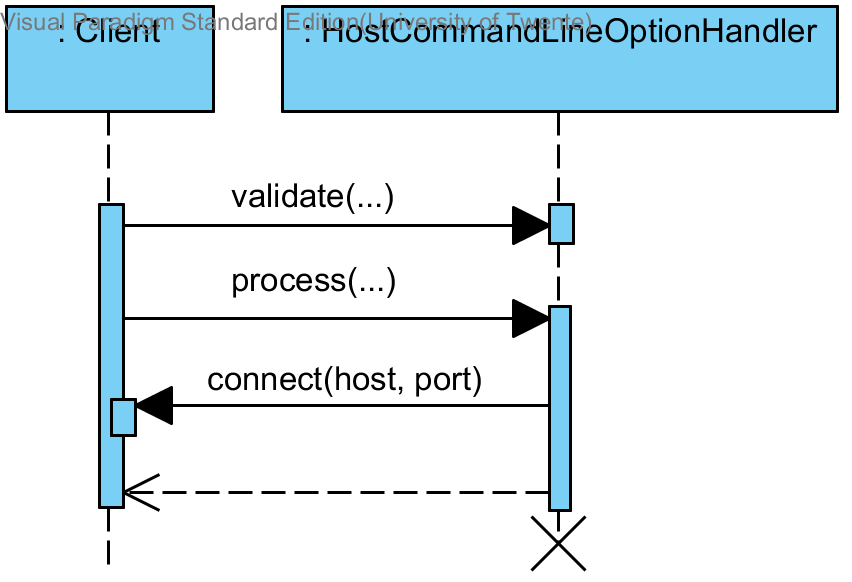
\includegraphics[width=0.36\textwidth]{diagrams/SD_client_host}
  \end{center}
  \vspace{-20pt}\caption{Simplified sequence diagram of the handling of the \lstinline{--host} command line option}\vspace{-15pt}
  \label{fig:sd_client_host}
\end{wrapfigure}

The first option that will be processed is the \lstinline{--host} option, which connects to the server. This is very straightforward and will requires no further elaboration. See \cref{fig:sd_client_host}.

Handling the model initializer option \lstinline{--model} is far more interesting. Several notable things are worth stating when looking at the sequence diagram in \cref{fig:sd_client_model} (\cref{app:sd}). Firstly, it can be seen that multiple model initializers can be selected. This is designed this way so the user can define the model in more than one way, perhaps even with the use of modules. In practise this can be used by simply passing the \lstinline{model} option multiple times. Multiple model initializers are executed in the same order as they were passed via the command line. Secondly, every model initializer should, of course, define the model with the initial state and the state-transitions. The initial state can be defined by defining the initial nodes and relations and adding them to the controller. This sends the information directly to the server. Each state-transition is defined as an instance of the \lstinline{ModelTransition} class and holds a \lstinline{groovy.lang.Closure} field. This is code that is executed when the transition is executed and should change the model to the next state. How the model initializer exactly defines the initial state and the state-transitions is up to the implementation (see \cref{sec:interfacedesign} for more on this). Finally, when the model initializers have been executed and thus the initial state has been defined, GreenMirror sends the "end transition" command to the server, indicating that the transition from state 0 (no state) to state 1 can be performed. 

Next in line is the handler for the \lstinline{--trace} option. See \cref{fig:sd_client_trace} (\cref{app:sd}) for the sequence diagram. This follows somewhat the same structure as the model initializer option handler, with a few slight differences. Only one \lstinline{TraceSelector} can be used. However, multiple \lstinline{ModelTransition}s can be executed with each transition from the trace, due to the fact that the \lstinline{ModelTransition} instance has a regular expression pattern that matches with zero to unlimited transitions from the trace. These transitions are executed in the order in which the model initializer added them to the controller. After each executed transition, GreenMirror sends an "end transition" command to the server, indicating that a new state has been reached. If the user wants GreenMirror to refrain from sending this command, perhaps because the executed transition is part of the previous or next one, the \lstinline{supplemental} flag of the \lstinline{ModelInitializer} instance can be set to true.

\begin{figure}[ht]
  \centering
  \makebox[\textwidth][c]{
  	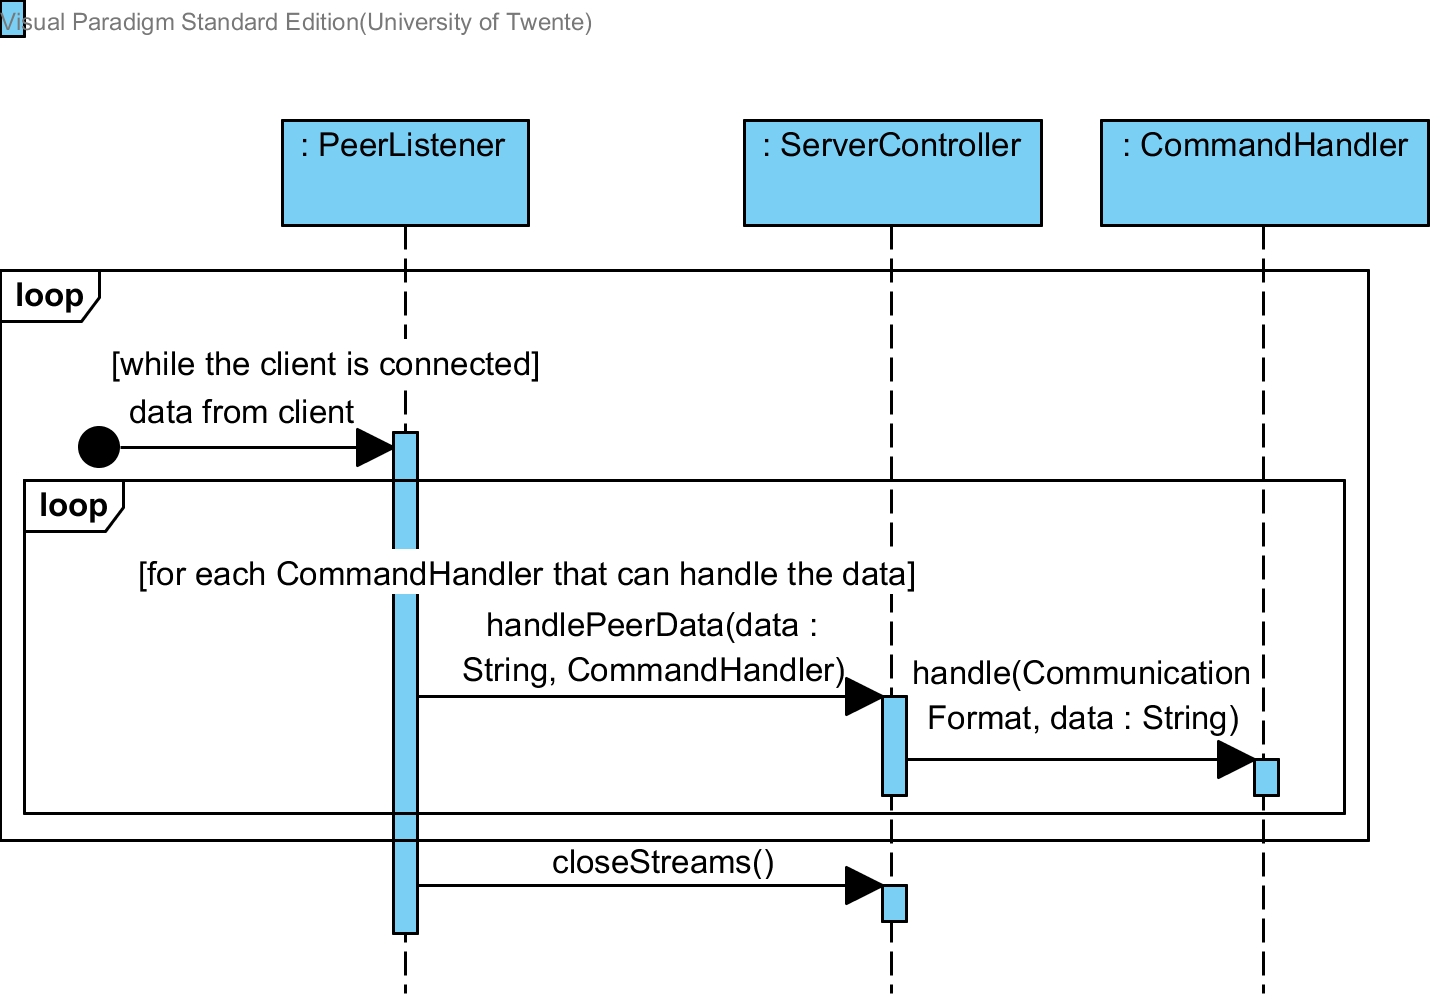
\includegraphics[width=0.6\textwidth]{diagrams/SD_server_receivecommand}
  }
  \caption{Simplified sequence diagram of the server receiving data}
  \label{fig:sd_server_receivecommand}
\end{figure}
The client is now finished and will close. In the meanwhile, the server has received the commands the server sent. Every command is passed to the correct \lstinline{CommandHandler} in the sequence as shown in \cref{fig:sd_server_receivecommand}. What exactly happens in the \lstinline{handle(CommunicationFormat, String)} method of the \lstinline{CommandHandler} entirely depends on the received command.

After the client has sent the "start visualization" command, the server starts the transition to the first state. Upon finishing, the correct toolbar buttons are enabled and the user can start interacting with the visualizer. What is seen in the sequence diagram of the user interaction (\cref{fig:sd_server_userinteraction} in \cref{app:sd}) is that all visualization parameters of the state-transition are derived from the button the user clicked on. More on this will be explained in \cref{subsec:implementationdetails}.


%--------------------------------
%----------------
%-------- Implementation details
%----
%--
\subsection{Implementation details}\label{subsec:implementationdetails}
Several implemented design choices and applied design patterns deserve more elaboration.

\subsubsection{State and state-transition tracking}\label{subsubsec:statetransitiontracking}
For future extensions, one of the most important parts to understand about the GreenMirror framework and application is the way it currently stores the state and state-transitions of the model internally. The client controller accepts changes in the model and immediately notifies the server of these changes. It also lets the server know when a state-transition ends, but it does not store the distinct states because this has no practical use in the current version (although it would be easy to implement by storing the state every time a \lstinline{ModelTransition} finishes execution). On the other hand, the server does have a practical use for storing the distinct states: the user can browse through the states. This, in combination with the fact that the main goal of the GreenMirror application is the visualization of state-transition models, results in the need for the server to store and track both the distinct states and the transitions between the states. Because storing different internal states of an object is a well-known programming scenario, the \emph{memento design pattern} (from \cite{kuchana2004,sourcemaking}) has been chosen to handle storing and restoring the visualizer states.

This pattern is implemented in the \lstinline{Visualizer} and \lstinline{VisualizerMemento} classes. Needless to say, \lstinline{VisualizerMemento} fulfils the memento role, encapsulating the state's nodes, their relations and the state-transition data to go to the next state. It should be noted that the current version does \emph{not} store the state's nodes and relations, because the way of storing state-transition data is sufficient. This can still be easily implemented in future versions if need be, due to the explicit use of the memento pattern: the \lstinline{Visualizer} class fulfils both the caretaker and originator roles, implementing the \lstinline{VisualizerMemento.Caretaker} and \lstinline{VisualizerMemento.Originator} interfaces to make this more expressive.

State-transition data is stored as instances of subclasses of the \lstinline{javafx.animation.Transition} class. Let's first expand some more on JavaFX' transition\footnote{note the distinction between JavaFX transitions and state-transitions. See \cref{subsec:glossary}} classes. JavaFX makes animated transitions very simple to implement. When defining one's own, \lstinline{javafx.animation.Transition} must be extended and only the \lstinline{interpolate(double)} method must be implemented. The argument of type \lstinline{double} is a fraction between zero and one, zero being 0\% and 1 being 100\%, indicating how far along the transition is. In this method, the value of the property that is animated should be set according to the fraction supplied by JavaFX and the starting and ending values of the property. There are several ready-made transitions available, such as \lstinline{FadeTransition} and \lstinline{RotateTransition}. JavaFX also has two special transitions: \lstinline{ParallelTransition} and \lstinline{SequentialTransition}. These play other transitions that are added to their lists in parallel or sequentially, respectively, and can be nested.

\begin{wrapfigure}{o}{0.38\textwidth}\vspace{-20pt}
  \begin{center}
    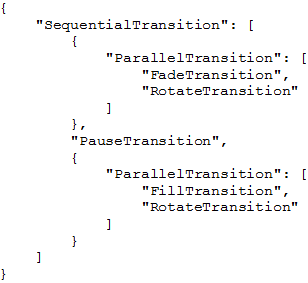
\includegraphics[width=0.36\textwidth]{diagrams/transitiontree}
  \end{center}
  \vspace{-10pt}\caption{An example of one stored state-transition in JSON notation}\vspace{-12pt}
  \label{fig:transitiontree}
\end{wrapfigure}
This is also how GreenMirror stores a state-transition: one \lstinline{SequentialTransition} holding one or multiple \lstinline{ParallelTransition}s (separated by a \lstinline{PauseTransition} to incorporate an optional delay) which in turn hold the individual \lstinline{Transition} instances that animate the change in properties. Initially, every change in the model the server receives ends up in the same \lstinline{ParallelTransition}. The user might want to show several sequential animations during one state-transition. For this scenario, the flush command has been implemented. This results in the server creating a new \lstinline{ParallelTransition} entry in the root \lstinline{SequentialTransition} in which all further transitions will be stored. For an example of these nested transitions of one state-transition, see \cref{fig:transitiontree}.

A reason to store only these \lstinline{Transition}s in the memento is the fact that reversing the animation of a \lstinline{Transition} is as easy as setting its \lstinline{rate} property to a negative value. This makes it simple to go back and forth between states without the need to recalculate property values of JavaFX nodes.


\subsubsection{\lstinline{FxWrapper} and \lstinline{FxPropertyWrapper}}\label{subsubsec:fxwrapper}
Each GreenMirror node that has a visual appearance needs to store and track the properties of its FX. This is done using the \emph{proxy design pattern} (see \cite{kuchana2004,sourcemaking}), with subclasses of the abstract \lstinline{FxWrapper} class. These subclasses are also loaded using the \lstinline{ServiceLoader} class. Using a wrapper in stead of directly using a JavaFX node instance has several reasons:
\begin{enumerate}
\item \lstinline{FxWrapper} provides general methods such as converting FX data into an object that can be shared between client and server, or changing general properties like the rotation and opacity of a JavaFX node.
\item The implementations of abstract methods of \lstinline{FxWrapper} used by GreenMirror might differ per type of JavaFX node. For example: the calculations of a specific placement on the edge of a circle differ from the calculations of a placement on the edge of a rectangle.
\item For the logic in the user's model and the proper creation of state-transitions on the server, properties have to be set and changed during the processing of state-transitions in the model without directly affecting the FX in the visualizer. As mentioned in \cref{subsubsec:statetransitiontracking}, changing actual properties of JavaFX nodes happens as a consequence of the execution of JavaFX transitions. To work with these values without directly visualizing them, a wrapping layer is needed providing 'virtual' values. 
\item Support for new types of JavaFX nodes can be easily added. Examples include ellipses, three-dimensional shapes and composite nodes.
\end{enumerate}
The abstract \lstinline{FxShapeWrapper} subclass adds support for JavaFX nodes that extend \lstinline{javafx.scene.shape.Shape}, such as the fill property.

As just stated, it is easy to implement support for the use and visualization of a new type of JavaFX node to the framework:
\begin{enumerate}
\item Create a new subclass of \lstinline{FxWrapper} or \lstinline{FxShapeWrapper}.
\item Implement all necessary methods and override the relevant ones.
\item Add the JavaFX node properties you want to support (see below).
\item Add the binary class name of the new subclass to \lstinline{META-INF/services/greenmirror.FxWrapper}.
\end{enumerate}

The way \lstinline{FxWrapper} converts its properties to an object that can be sent over the network, is generalized in the sense that support for new types of properties can also be implemented easily. This will be clarified with an example. One of the supported properties of \lstinline{ImageFxWrapper} is the X coordinate of type \lstinline{double}. In the current GreenMirror version, FX data is sent to the server in JSON format (more on this in \cref{subsubsec:communication}). The value of the X coordinate can be easily converted to and from a string format, as would the boolean-type \lstinline{preserveRatio} property. So how would the \lstinline{image} property of type \lstinline{javafx.scene.image.Image} be converted to and from a valid JSON string? To make this modular and easily extendible, the abstract \lstinline{FxPropertyWrapper} class handles this, also implementing the proxy design pattern. Adding support for properties to an \lstinline{FxWrapper} now becomes more general and easy and results in these steps:
\begin{enumerate}
\item If no \lstinline{FxPropertyWrapper} exists yet for the type of the property, create and implement it.
\item Add the property to \lstinline{getAnimatableProperties()} if it can be animated or to \lstinline{getChangableProperties()} if it can only be set once. These two methods are the overridden ones in the \lstinline{FxWrapper} subclass the property belongs to.
\item Add one or more get-methods to the \lstinline{FxWrapper} subclass.
\item Add one or more set-methods to the \lstinline{FxWrapper} subclass. The type of the argument of the primary set-method depends on what the relevant \lstinline{FxPropertyWrapper}'s \lstinline{getPropertyType()} method returns.
\item If the property can be animated, but hasn't got a \lstinline{javafx.animate.Transition} implementation yet, create it. The abstract \lstinline{AbstractTransition} and \lstinline{DoublePropertyTransition} classes have been created to provide several often used methods when extending \lstinline{javafx.animate.Transition}.
\item If the property can be animated, add the animate method that returns the \lstinline{Transition} that changes the value of the property when played.
\item If the user needs access to the new property type in the Groovy model initializer (which will be explained in \cref{sec:interfacedesign}), add an import to\\ \lstinline{greenmirror.client.modelinitializers.GroovyScriptModelInitializer#IMPORTS}.
\end{enumerate}

From the above description and \cref{subsubsec:statetransitiontracking}, one might realize that this design has a notable constraint: JavaFX node properties that are changed after they are initially set \emph{must} be animatable. However, the obstacle of animating the change of a discrete property can be overcome by implementing  a \lstinline{Transition} that animates a fade-out, changes the value, and animates a fade-in to the original opacity. This solution is used to animate changes in the image property of \lstinline{ImageFxWrapper} and the text property in \lstinline{TextFxWrapper}.



\subsubsection{Communication between client and server}\label{subsubsec:communication}
The abstract \lstinline{Command} and \lstinline{CommandHandler} classes respectively construct and interpret data exchanged between the client and the server. Every \lstinline{Command} instance received the necessary data in its constructor, remembers it and optionally performs some preparation before the controller requests the data as a string, formatted according to the set \lstinline{CommunicationFormat}. Currently, the JSON format is used. The controller prepends the name of the command before the data, so the peer on the receiving end knows which \lstinline{CommandHandler} to use.

In the current version, only communication from the client to the server is required. The server works on the basis of its received commands. This means two things. In theory, the server could get completely different functionalities, based on new implementations of \lstinline{CommandHandler}s. Secondly, the server must receive the initialization command before any other command that does something with the visualizer. In the current design this is the responsibility of the client, and specifically the model initializer implementations. New implementations of \lstinline{CommandHandler} can be added by adding them to the \lstinline{ServiceLoader} (by adding them to \\ 
\lstinline{META-INF/services/greenmirror.CommandHandler}) and making sure the implementation has at least one of the \lstinline{@ServerSide} or \lstinline{@ClientSide} annotations, indicating on which side the \lstinline{CommandHandler} should be used.



\subsubsection{Placement of nodes with respect to other nodes}\label{subsubsec:placement}
As already mentioned, placement relations between nodes indicate that one node of the relation, node A, is placed in a specific respect to the other node of the relation, node B. There are currently several extensions of the abstract \lstinline{Placement} class implemented which are described below and are illustrated in \cref{fig:placements}. Every instance of \lstinline{Placement} also has an optional  position relative to placement. For example: if a node A has an \lstinline{edge_top} placement with relative position \lstinline{(0, -20)} on node B, node A is placed 20 pixels above (and centred on) the edge of node B.

\begin{description}
\item[\texttt{Corner*Placement}] A placement on any of the corners of a JavaFX node: top left, top right, bottom right or bottom left.
\item[\texttt{Edge*Placement}]  A centred placement on any of the edges of a JavaFX node: top, right, bottom or left.
\item[\texttt{MiddlePlacement}] A placement in the exact middle of a JavaFX node.
\item[\texttt{EdgePlacement}]   A placement on the edge of a JavaFX node, according to a specified angle. An angle of zero degrees is the equivalent an \lstinline{edge_top} placement, and an angle of 90 degrees (positive) is the equivalent of an \lstinline{edge_right} placement. 
\item[\texttt{CustomPlacement}] A placement where only the relative position data is used to determine the coordinates. The relative position data is relative to the coordinates calculated for the \lstinline{MiddlePlacement}.
\item[\texttt{RandomPlacement}] A random placement on a JavaFX node. Upon receiving this placement data, the server replaces this with a \lstinline{CustomPlacement} where the relative position is set to the calculated, relative coordinates of the \lstinline{RandomPlacement}.
\item[\texttt{NoPlacement}] The default for a relation.
\end{description}

\begin{figure}[!ht]
  \centering
  \makebox[\textwidth][c]{
  	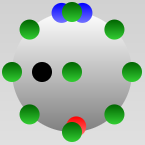
\includegraphics[width=0.25\textwidth]{images/placements}
  }
  \caption{An example available placements on a circle FX node. The green circles have a corner* (or at least, what would have been the corner), edge* or middle placement, the blue ones an edge placement with -10 and 10 degrees, the black one a custom placement with relative position \lstinline{(-10, 0)} and the red one a random placement.}
  \label{fig:placements}
\end{figure}
Every type of \lstinline{FxWrapper} must calculate the exact coordinates of a specific placement. The \lstinline{FxWrapper} class provides a static method to calculate these coordinates for a rectangle, given the width and height.

These placements are an important aspect of the visualization of nodes and their relations. They make sure the user doesn't have to work with actual coordinates in his model, except while defining the initial state, thus they provide a level of abstraction. Although the current implementations offer often used placements, a developer might want to add more distinct ones. This can be done by adding his implementation to \lstinline{META-INF/services/greenmirror.Placement} so it can be loaded by \lstinline{ServiceLoader}, and by adding the proper calculations to every \lstinline{FxWrapper} type.

\subsubsection{The visualizer's playback states}\label{subsubsec:playbackstates}
\begin{wrapfigure}{o}{0.38\textwidth}\vspace{-12pt}
  \begin{center}
    
\includegraphics[width=0.36\textwidth]{images/toolbar_paused_withsiblingstates}
  \end{center}
  \vspace{-10pt}\caption{The toolbar when the visualizer is in the paused playback state and has previous and next model states}\vspace{-12pt}
  \label{fig:toolbar}
\end{wrapfigure}

After the visualizer has been initialized, it can be doing one of three things: it can be waiting for the model to load, it can be waiting for the user to interact, or it can be playing an animation. The latter two will be discussed here. Note the explicit difference between the model's state and the visualizer's playback state.

From \cref{fig:sd_server_userinteraction} (discussed in \cref{subsec:detailedworkflow}) can be seen that the operation of the different toolbar buttons is determined directly after the playback state has been changed. This means that the behaviour of a button depends on the playback state (and the availability of a previous or next model state), resulting in the use of the \emph{state design pattern} (see \cite{kuchana2004,sourcemaking}). Every playback state has its own class that implements the \lstinline{Visualizer.PlaybackState} interface.

A reciprocal action can also be seen in \cref{fig:sd_server_userinteraction}: when the user clicks a button, the playback state changes. This changes the playback state as illustrated in the state machine diagram of \cref{fig:smd_playbackstates}. As one might notice, there are five states in \cref{fig:smd_playbackstates}, but seven buttons in \cref{fig:toolbar}. This is because the most left and most right buttons respectively rewind and forward through the model states. These result in a "stepping" playback state, with the difference that the JavaFX transition is played with a highly increased speed to make them nearly instantaneous.
\begin{figure}[H]
  \centering
  \makebox[\textwidth][c]{
  	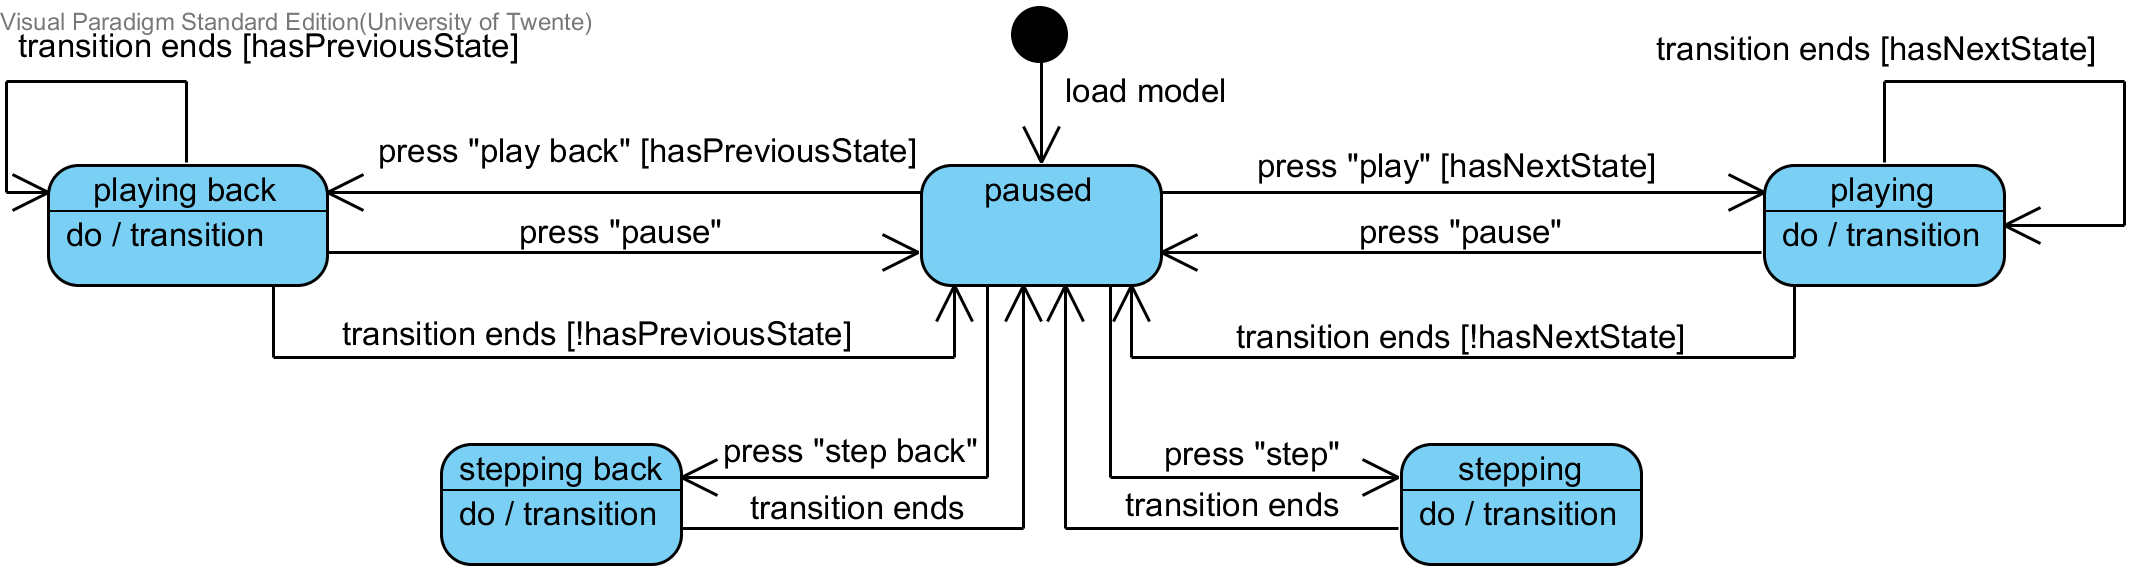
\includegraphics[width=0.95\textwidth]{diagrams/smd_playbackstates}
  }
  \caption{The state machine diagram for the playback states}
  \label{fig:smd_playbackstates}
\end{figure}


\subsubsection{Miscellaneous}\label{subsubsec:misc}
A singleton \lstinline{Log} class is available that accepts any implementation of \lstinline{PrintStream} as its output by way of the \emph{strategy design pattern} (see \cite{kuchana2004,sourcemaking}). Multiple can be used simultaneously and are selected at the entry point of the respective client and server. The client doesn't have a visual user interface, so it only selects the default \lstinline{System.out}. The server is mainly visual, so it uses both the default \lstinline{System.out} and the GreenMirror \lstinline{WindowLogger} class to create a window that shows the log entries (see \cref{fig:log}). Log entries are prefixed with a time stamp, including the milliseconds so the timing can also be analysed. The log also has a verbose setting: when set to true, a lot more information is provided about what exactly is happening internally.
\begin{figure}[H]
  \centering
  \makebox[\textwidth][c]{
  	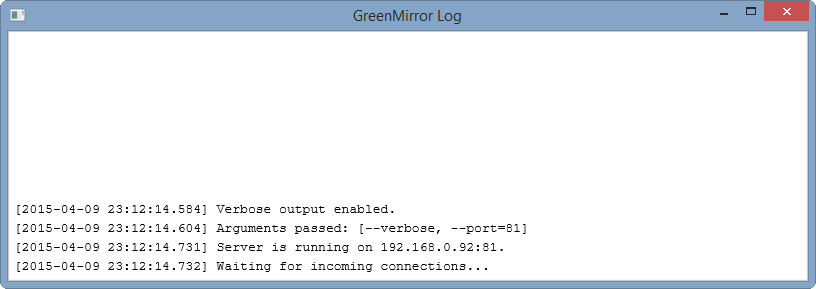
\includegraphics[width=0.95\textwidth]{images/log}
  }
  \caption{An instance of the \lstinline{WindowLogger}}
  \label{fig:log}
\end{figure}

When a state-transition removes a JavaFX node from the visualizer, it doesn't actually gets removed internally. It would be a hassle to remove and re-create the JavaFX node each time the user respectively reaches the states and comes back to it. This would also cause several other difficulties, such as the fact that GreenMirror needs to know that a JavaFX node has to be added \emph{before} it transitions back to the state (so it can animate the creation). That's why JavaFX nodes are not actually removed: they are merely made invisible by changing the opacity to zero. However, in anticipation of future extensions, the JavaFX nodes are also made untouchable for mouse events. This way, invisible nodes don't become an invisible layer preventing mouse events on other nodes. Before the start of each JavaFX transition, GreenMirror checks if the JavaFX transition tree contains a \lstinline{FadeTransition} that fades a JavaFX node in from an opacity value of zero. If so, it sets the visibility property to true. After a JavaFX transition has ended, it checks if the JavaFX transition tree contains a \lstinline{FadeTransition} that faded a JavaFX node to opacity value zero. If so, it sets the visibility property to false, making it practically not there as far as the user knows.
When a GreenMirror node is removed in the model of the client, it is replaced by an instance of \lstinline{NullNode}, following the \emph{null object design pattern} (see \cite{kuchana2004,sourcemaking}). This makes sure the model throws expected exceptions and ensures the user will get properly notified if he tries to access it.

\begin{wrapfigure}{o}{0.25\textwidth}\vspace{-22pt}
  \begin{center}
    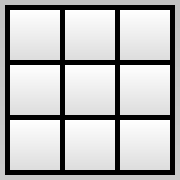
\includegraphics[width=0.23\textwidth]{images/grid}
  \end{center}
  \vspace{-10pt}\caption{The result of the \lstinline{GridBuilder} example code of \cref{lst:gridbuilder}}\vspace{-20pt}
  \label{fig:grid}
\end{wrapfigure}
GreenMirror has an auxiliary \lstinline{GridBuilder} class created to take away the tedious work of building a grid of nodes. As one might guess, it follows the \emph{builder design pattern} (see \cite{kuchana2004,sourcemaking}). It supports properties such as the amount of cells, the cell width and height, cell spacing, cell colour, borders, a background colour and the type and name prefix for every GreenMirror node it creates. It builds the grid by creating a GreenMirror node per cell and one extra for the background, all of which have \lstinline{RectangleFxWrapper}s. \Cref{lst:gridbuilder} Shows an example of how short the code is to create a TicTacToe grid, in contrast to defining every single GreenMirror node, not to mention the tedious work of getting their exact positioning right. The result result is visible in \cref{fig:grid}.
\begin{lstlisting}[language=Java, label={lst:gridbuilder}, caption={Example code to build a grid of nodes}]
new GridBuilder("ticTacToeGrid:cell_")
    .setCellCount(3, 3)
    .setCellSize(50, 50)
    .setCellFill("linear-gradient(to bottom, #FFF, #DDD)")
    .setCellSpacing(5)
    .setBorderSize(5) // top, right, bottom and left
    .setBackgroundFill("black")
    .build(10, 10) // Coordinates on the visualizer
    .getNodes()
\end{lstlisting}

Although both the client and the server work with multiple threads, there is no need for extensive measures to ensure thread safety. As the client currently does not receive data from the server, everything is executed on the main thread. The server, on the other hand, does work with a JavaFX thread and a \lstinline{PeerListener} thread. However, seeing as the JavaFX thread starts visualizing after the complete model has been received from the client, and the user interaction with the visualizer is limited during visualizations (as is explained in \cref{subsubsec:playbackstates}), no concurrency can occur.


%%% Why Java?








%----------------------------------------------------------------------------------------
%------------------------------------------------
%------------------------ Interface design
%-------------
%------
\section{Interface design}\label{sec:interfacedesign}
This section discusses the available interfaces for tool owners that provide ways of loading models into GreenMirror, and the current implementations. Loading a model consists of two parts: defining the model and providing the trace that defines in which order state-transitions will take place. Both parts have corresponding interfaces, respectively \lstinline{ModelInitializer} and \lstinline{TraceSelector}, and the usage of the implementations follows the \emph{strategy design pattern} (see \cite{kuchana2004,sourcemaking}).

The model initializer has a few responsibilities. First and foremost it must, in the most general sense and not surprisingly, initialize the model according to the specifications of the user. More specifically: it must receive information from the user about how the initial state of the model is defined and how different state-transitions influence the model and the visualization. How the model initializer receives this information is up to the implementation. Once it has received this information, it can add nodes to the \lstinline{Client} controller, remove nodes, etcetera. These changes are automatically conveyed to the server. The model initializer can also use the interface with the controller to send commands directly to the server, by use of the currently available commands in the \lstinline{greenmirror.commands} package. It is not recommended that the model initializer uses this to directly convey model changes, because this circumvents the logic incorporated in updating the model via the controller. It is meant to provide the possibility to send auxiliary commands such as the \lstinline{SetAnimationDurationCommand}, which sets the duration of all animations created as a result of upcoming model changes.

The model initializes should define what model changes should happen by adding a new instance of \lstinline{ModelTransition} to the controller. As mentioned in \cref{subsec:detailedworkflow}, this class has a \lstinline{groovy.lang.Closure} field that changes the model when executed. This is type is chosen to directly support the first implemented model initializer (discussed below), although it is not restricted to the first implementation. The closure can accept arguments based on the trace transition. This is best explained using an example. Suppose the user wants to visualize a ConnectFour game. It would be unwieldy to define a state-transition for every possible move (although there are only seven at the most), so the user defines one state-transition that uses the regular expression \lstinline{^move(\d+)$} to accept transitions from a trace. This means it needs the number of the column as an argument in the closure that executes the state-transition. Fortunately, the Groovy library supports this and GreenMirror takes advantage of this by supporting string and integer type arguments.

As mentioned in \cref{subsubsec:communication}, the server could be completely re-purposed by implementing and using different \lstinline{Command}s and \lstinline{CommandHandler}s. However, if the server will be used as a visualizer, the model initializer has the responsibility of making sure the server first receives the initialization command. Without it, there is no JavaFX stage to which JavaFX nodes can be added. Of course, the implemented model initializer could delegate this responsibility to the user.

The model initializer that has been implemented in this first version of GreenMirror is based on Groovy (see \cite{groovy}). Groovy is a dynamic language for the Java platform and provides a vast array of useful features. Specifically, the model initializer uses Groovy's script functionalities. This choice was made due to the following reasons.
\begin{enumerate}
\item The user receives the power and flexibility of a full-featured programming language, but still is easy to learn. This means that both advanced programmers and users without much experience can use it.
\item The user scripts can be executed during runtime, meaning that, while employing a complete programming language, the GreenMirror framework doesn't have to be recompiled every time the user selects a different model.
\item A clear interface with the controller can be provided to the user, which Groovy calls a \emph{base class}. The user can refer in his script to the base class' methods without referring to any object. This works as if the user is programming in the context of one of the methods of the base class (which it also comes down to, internally).
\end{enumerate}
\Cref{lst:groovyexample} shows an example of a user script that can be executed by the \lstinline{GroovyScriptModelInitializer}. \Cref{fig:groovyexample} shows a screenshot of its resulting visualization. It can be seen from the listing that chained statements are possible and actually encouraged to improve the readability of the script. Another notable advantage is that it is easily seen that calls to the base class (and thus indirectly to the controller) indicate a read from or a write to the model. For example, creating a new \lstinline{Node} instance does not mean it is added to the model. \lstinline{addNodes()} takes care of that.
\begin{lstlisting}[language=java, label={lst:groovyexample}, caption={Example Groovy user script}]
initialize(600, 400);
addNodes(
    new Node("loc:1").set(fx("rectangle")
                          .setSize(200, 400).setPosition(0, 0)
                          .setFill("radial-gradient(center 100px 200px, "
                                                 + "radius 200px, white, red)")),
    new Node("loc:2").set(fx("rectangle")
                          .setSize(200, 400).setPosition(400, 0)
                          .setFill("radial-gradient(center 500px 200px, "
                                                 + "radius 200px, white, red)")),
    new Node("obj").set(fx("circle")
                          .setRadius(20)
                          .setFill("linear-gradient(to bottom, "
                                 + "limegreen, black)"))
);
addRelation(
    new Relation("on").setNodeA(node("obj"))
                      .setNodeB(node("loc:1"))
                      .setPlacement(Placement.MIDDLE)
);

addTransition("switch", {
    switchPlacementRelation(
        node("obj").getPlacementRelation().clone()
                                          .setNextNodeB(nodes("loc:"))
    );
});
\end{lstlisting}
\begin{figure}[H]
  \centering
  \makebox[\textwidth][c]{
  	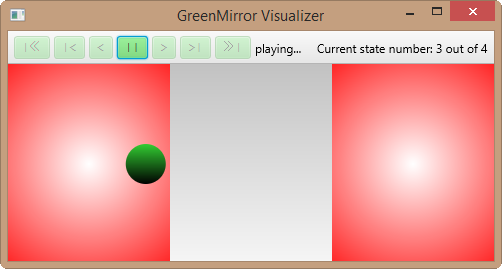
\includegraphics[width=0.8\textwidth]{images/groovyexample}
  }
  \caption{A screenshot of the executing visualization of \cref{lst:groovyexample} with trace \lstinline{switch}, \lstinline{switch}, \lstinline{switch}}
  \label{fig:groovyexample}
\end{figure}

After the model initializer has set the initial model state and saved all \lstinline{Model-transition}s, the selected \lstinline{TraceSelector} gets executed. \Cref{subsec:detailedworkflow} already elaborated on the sequence of events in which a \lstinline{TraceSelector} is executed. The current \lstinline{FileTraceSelector} implementation retrieves the trace from a simple file where the transitions are separated by a newline. In the visualization example of \cref{fig:groovyexample}, the trace file looked like \cref{lst:traceexample}. In the toolbar of \cref{fig:groovyexample} a state count of four can be seen, while three transitions are in the trace. This is naturally because the initial state is included in the count.	
\begin{lstlisting}[label={lst:traceexample}, caption={Example trace file}]
switch
switch
switch
\end{lstlisting}
Both the \lstinline{ModelInitializer} and \lstinline{TraceSelector} interfaces accept one argument from the command line. This should be the source of the model and trace, respectively. In \lstinline{GroovyScriptModelInitializer} this is the file name of the Groovy script, while in \lstinline{FileTraceSelector} this is the name of the file containing the trace. In future implementations that, for example, connect GreenMirror to another tool, this could be the name of the model.








\newpage
%----------------------------------------------------------------------------------------
%------------------------------------------------
%------------------------ Validation
%-------------
%------
\section{Validation}\label{sec:validation}
\begin{wrapfigure}{o}{0.3\textwidth}\vspace{-22pt}
  \begin{center}
    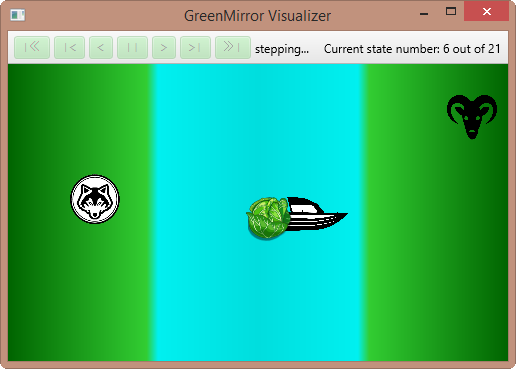
\includegraphics[width=0.28\textwidth]{images/ferryman}
  \end{center}
  \vspace{-10pt}\caption{A screenshot of the visualized ferryman puzzle}\vspace{-10pt}
  \label{fig:ferryman}
\end{wrapfigure}
Due to the visual nature of the application, most tests are based on visual inspection. Several unit tests have been written using the JUnit library. These test the essential model classes used by the client and server: \lstinline{Node}, \lstinline{Relation}, \lstinline{NodeList} and \lstinline{RelationList}. Furthermore, the \lstinline{FxWrapper} class and its currently implemented subclasses have been unit-tested to validate their correct functioning with the client. In addition to these subclasses, a separate unit test has been written to validate the calculations used for the placements per \lstinline{FxWrapper} type. The proper functioning of these classes is essential for the user to be able to create a model that can be researched with GreenMirror.

\begin{wrapfigure}{i}{0.3\textwidth}\vspace{-22pt}
  \begin{center}
    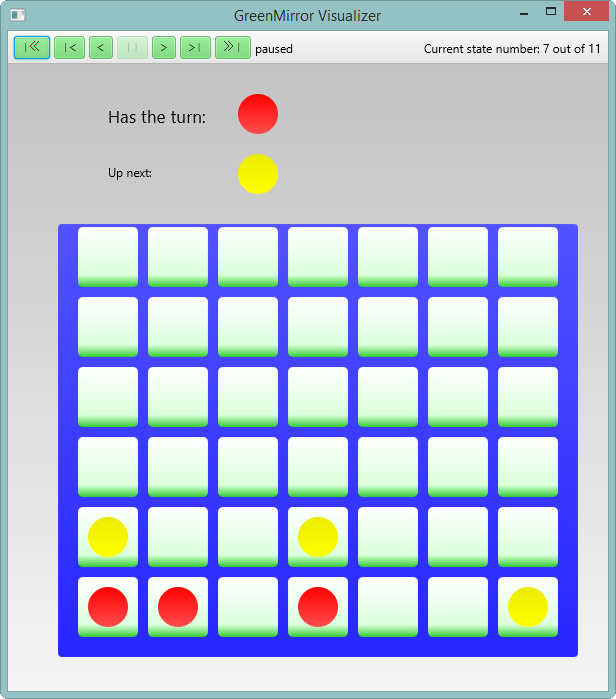
\includegraphics[width=0.28\textwidth]{images/connectfour}
  \end{center}
  \vspace{-10pt}\caption{A screenshot of the visualized ConnectFour game}\vspace{-10pt}
  \label{fig:connectfour}
\end{wrapfigure}

Other validation tests have been done with the \lstinline{GroovyScriptModelInitializer} using comprehensive Groovy scripts. These scripts enable the user to validate the workings of GreenMirror by inspecting the visual results. The Groovy scripts \lstinline{testcases/systemtest1.java} and \lstinline{testcases/systemtest2.java} located on the repository of this project, together with their respective trace files found in the same directory, extensively validate the possibilities of GreenMirror. They include tests from simply adding nodes and relations in all possible ways, to moving multiple chained, rigidly placed nodes around.

A few test models were described in \cref{subsec:requirementsvalidation}. These were also used as system tests and are also available in the \lstinline{testcases} directory on the repository. Screenshots of the resulting visualizations can be found in \cref{fig:ferryman,fig:connectfour,fig:phil} for the ferryman puzzle, the ConnectFour game and the Dining Philosophers problem, respectively.

\begin{figure}[ht!]
  \makebox[\textwidth][c]{
  	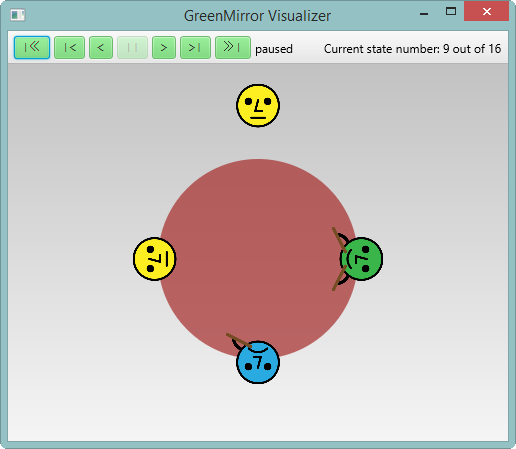
\includegraphics[width=0.8\textwidth]{images/phil}
  }
  \centering
  \caption{A screenshot of the visualized Dining Philosophers problem}
  \label{fig:phil}
\end{figure}
~ % hard space because else there is nothing between the above image and the upcoming section header, resulting in the section header being centred due to the \centering operation of the above image.

%--------------------------------
%----------------
%-------- Metrics
%---- (Only added if there is relevant data about the metrics.)
%--
%\subsection{Metrics}


%----------------------------------------------------------------------------------------
%------------------------------------------------
%------------------------ Discussion
%-------------
%------
\section{Discussion}\label{sec:discussion}
The GreenMirror application is the first step in the creation of an extensive research tool. This section will discuss several ideas for future improvements. First and foremost, it should be stated that future versions should be designed or altered into a more modular and structured way and by a more experienced developer. Although the current version does fulfil its intended purpose, the framework hasn't even begun to reach its full potential.

The log functionalities could be extended and modified to present event data in a more structured way. Several event 'levels' could be added, such as regular messages, warnings and fatal errors. To use the log as a proper debug tool for the researched model, snapshots of the system state could be included, possibly in an additional output sink.

To make the client more user friendly to work with, a graphical interface could be added. This is in no way necessary with the current functionality. It would just provide more convenience for the user and would be more appealing for the eye.

A caching function on the server might result in a slight performance improvement when handling models consisting of over hundreds of state-transitions. The performance improvement would reside in the fact that the trace selector wouldn't have to process all state-transitions every time the model is loaded, but it would retrieve the already-constructed animations and states from a cache file. This also means that every time the client knows it's going to process a model, it sends a checksum of the model and the trace to the server, verifying if processing is necessary at all. The user would in practice alter his model or trace a lot, which raises the question how often this caching function would be used.

JavaFX has extensive 3D visualization possibilities. These could provide more eye-appealing visualizations for the simple models presented in this report, but could also be an essential asset in visualizing more complex models. The current version of GreenMirror already supports the extra z-coordinate by working with \lstinline{javafx.geometry.Point3D} objects in stead of \lstinline{javafx.geometry.Point2D} objects to represent positions on the visualizer . A developer could fairly easily extend the framework so it can work with 3D shapes. Together with some other small modifications, this can be accomplished implementing new \lstinline{FxWrapper} and \lstinline{Placement} subclasses.

There is currently a \lstinline{TraceSelector} implementation in development by the Formal Methods and Tools research group of the University of Twente to select a trace from the Groovy application. A next improvement to GreenMirror could be the development of a \lstinline{ModelInitializer} implementation that can load a model from an existing GROOVE Grammar. This would narrow the bridge between the two tools and would certainly be considered a useful functionality. Should such an implementation be developed, the user might be required to provide extra information about how GROOVE's nodes should be represented on the visualizer. Fortunately this can be done rather simple: the user can provide a script that uses the Groovy \lstinline{ModelInitializer} implementation to supplement the model, which is possible because multiple model initializers can be used in GreenMirror.

Continuing this line of thought: why not write a supplement to the Groovy model initializer that constructs a GROOVE model (or model for another tool) from the model the user defines in his script? This would not be easy due to the different ways the tools work, but shouldn't be impossible. This way, a model could be analysed by writing it just one time in stead of writing it two times for two different tools.

To conclude this section some recommendations must be given to the developers and researchers that might want to further develop the GreenMirror framework. First, future developers should take a critical look at the degree of structure implemented in the design of the framework and specifically whether it is sufficient for future development. Secondly, as is discussed in \cref{subsec:possibleextensions}, it is a very large project to develop extensive support for generating a model based on interaction with the visualizer. Therefore, the suggestion is to first, or perhaps rather in parallel, develop implementations of \lstinline{ModelInitializer} and \lstinline{TraceSelector} to connect other tools to GreenMirror.






%----------------------------------------------------------------------------------------
%------------------------------------------------
%------------------------ References
%-------------
%------
\bibliographystyle{plain}
\bibliography{bibliography}





%----------------------------------------------------------------------------------------
%------------------------------------------------
%------------------------ Appendices
%-------------
%------
\appendix

\begin{comment}
\newpage\section{Class diagrams}\label{app:cd}
\end{comment}

\newpage\section{Activity diagrams}\label{app:ad}

\begin{figure}[ht]
  \makebox[\textwidth][c]{
  	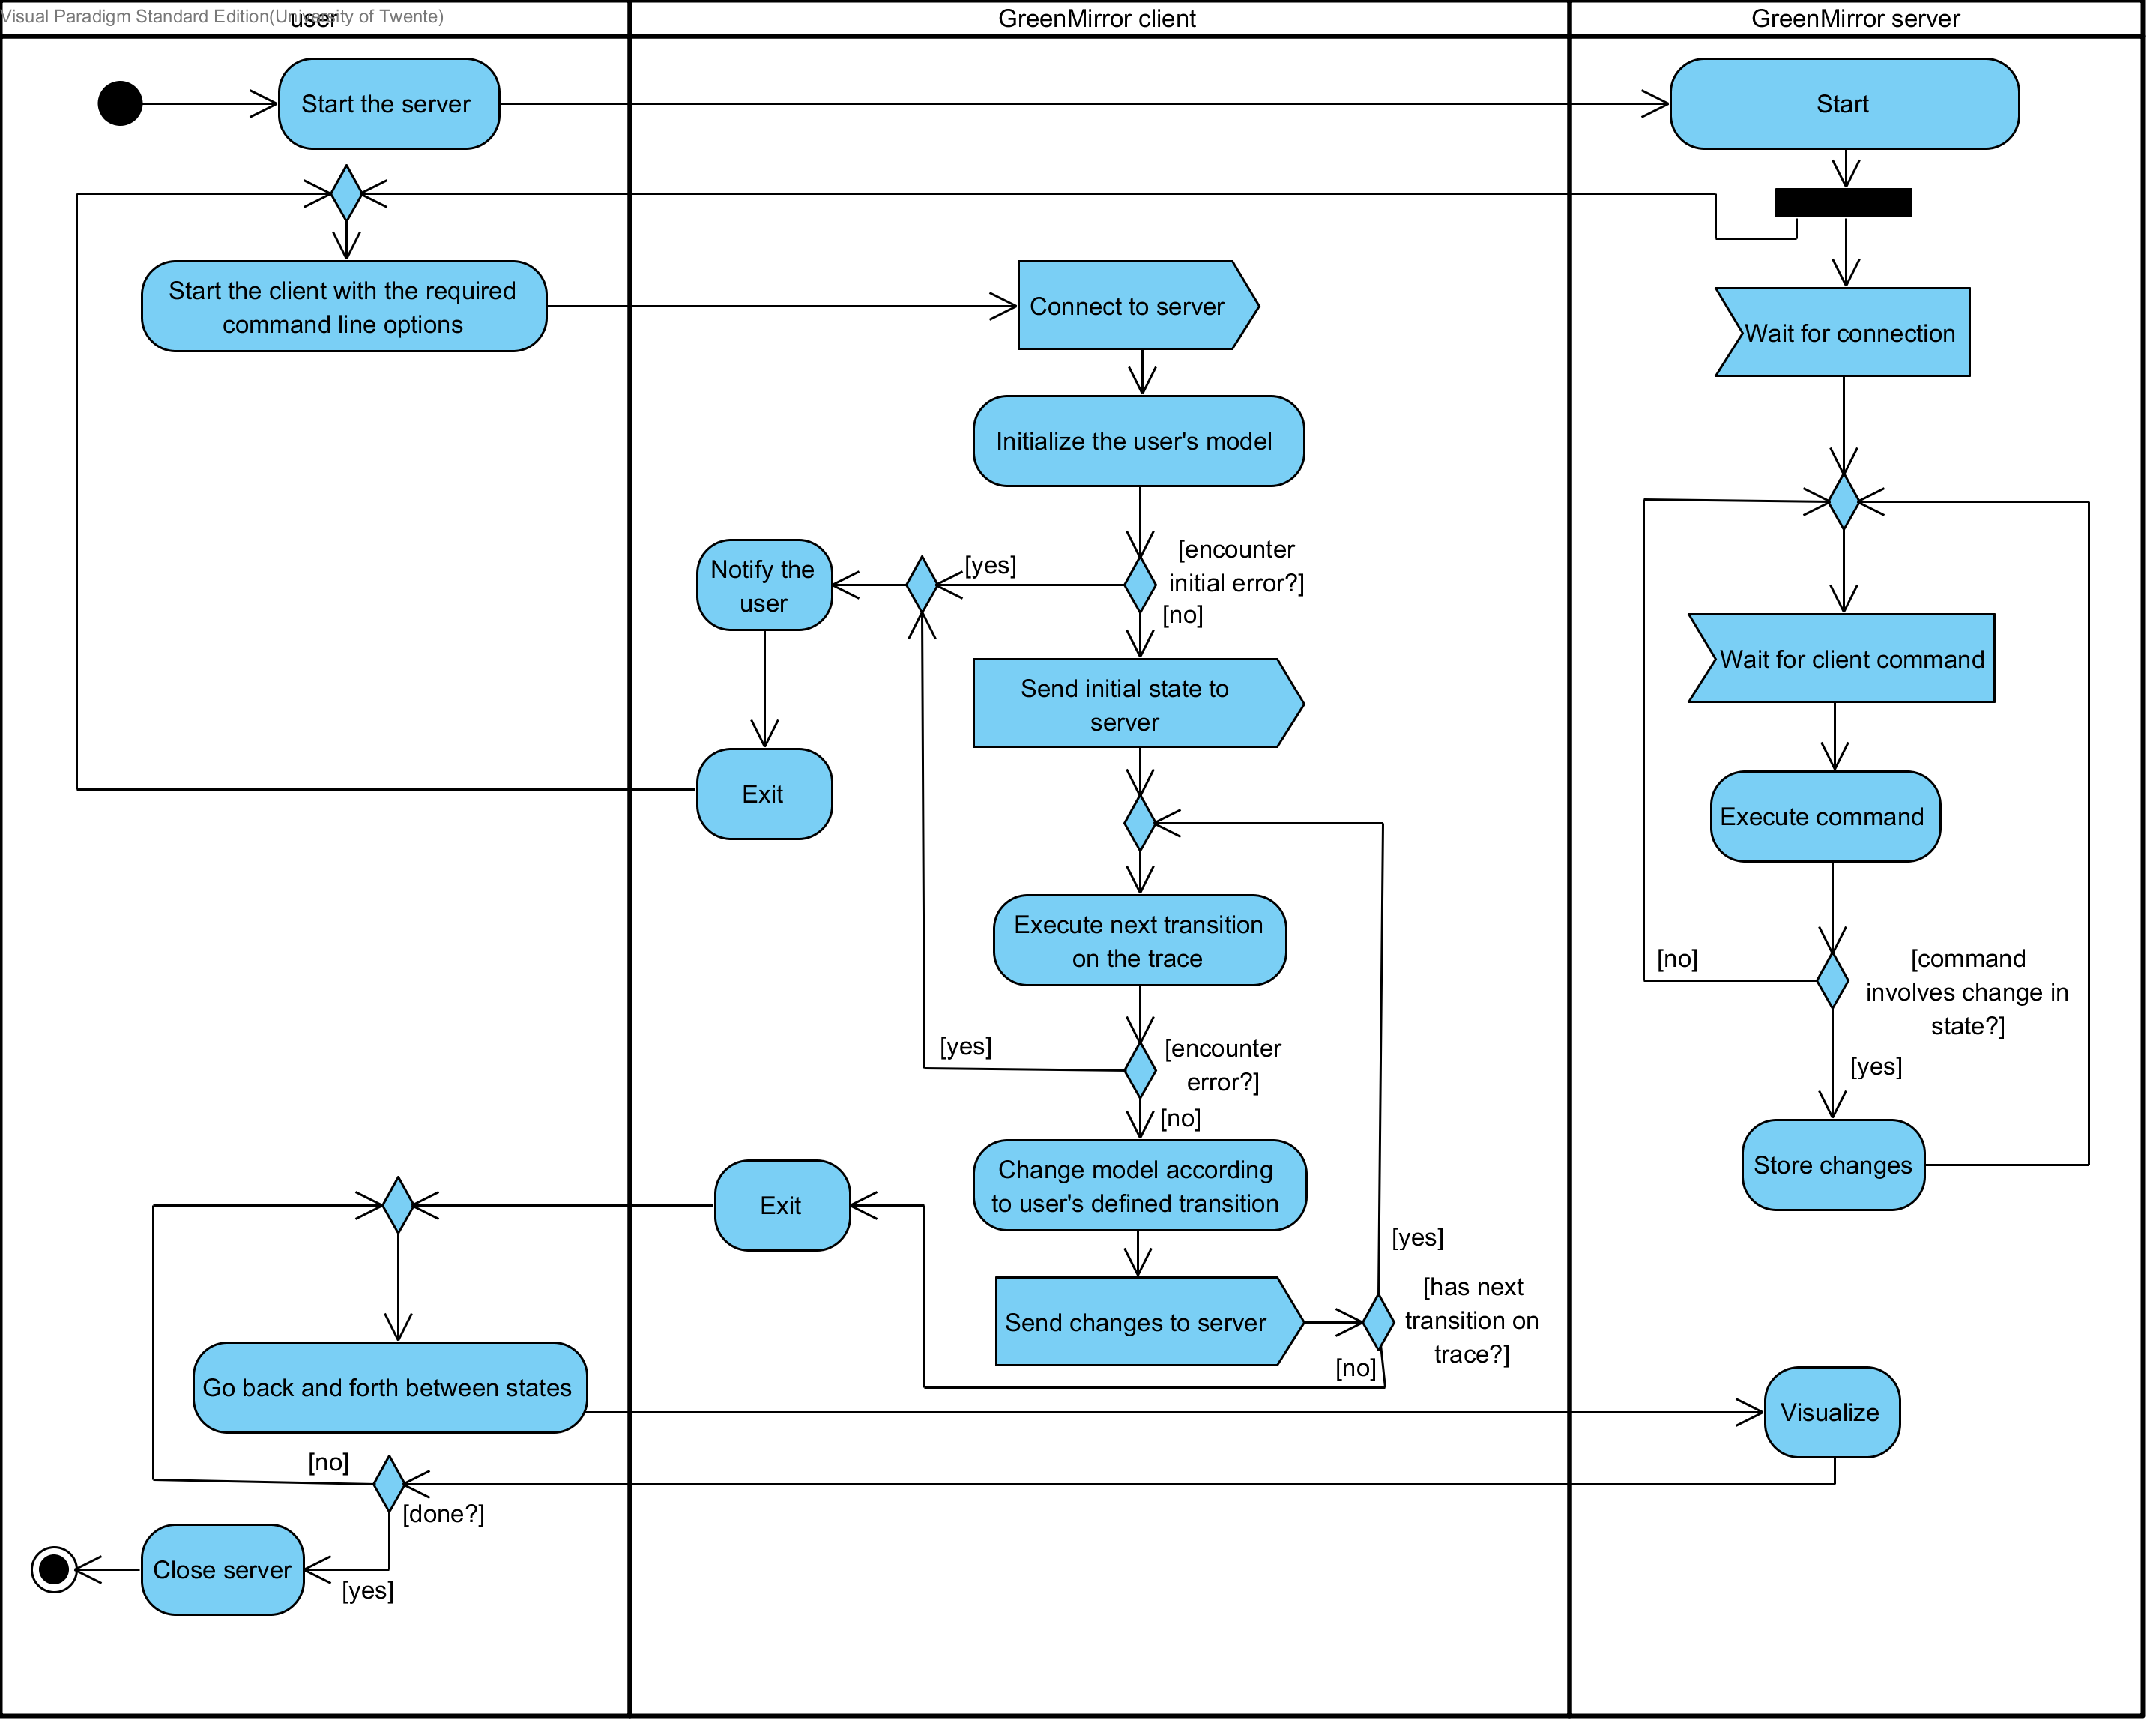
\includegraphics[width=1.3\textwidth]{diagrams/AD_generalworkflow}
  }
  \caption{Simplified activity diagram of the general work-flow}
  \centering
  \label{fig:app:ad_generalworkflow}
\end{figure}



\newpage\section{Sequence diagrams}\label{app:sd}
All diagrams are simplified in the sense that they do not show every atomic operation and that they show only validation and error handling when it is relevant and essential to the understanding of the sequences. They are simplified to improve the overall orderliness and comprehensibility of the diagrams.
\begin{figure}[hb]
  \centering
  \makebox[\textwidth][c]{
  	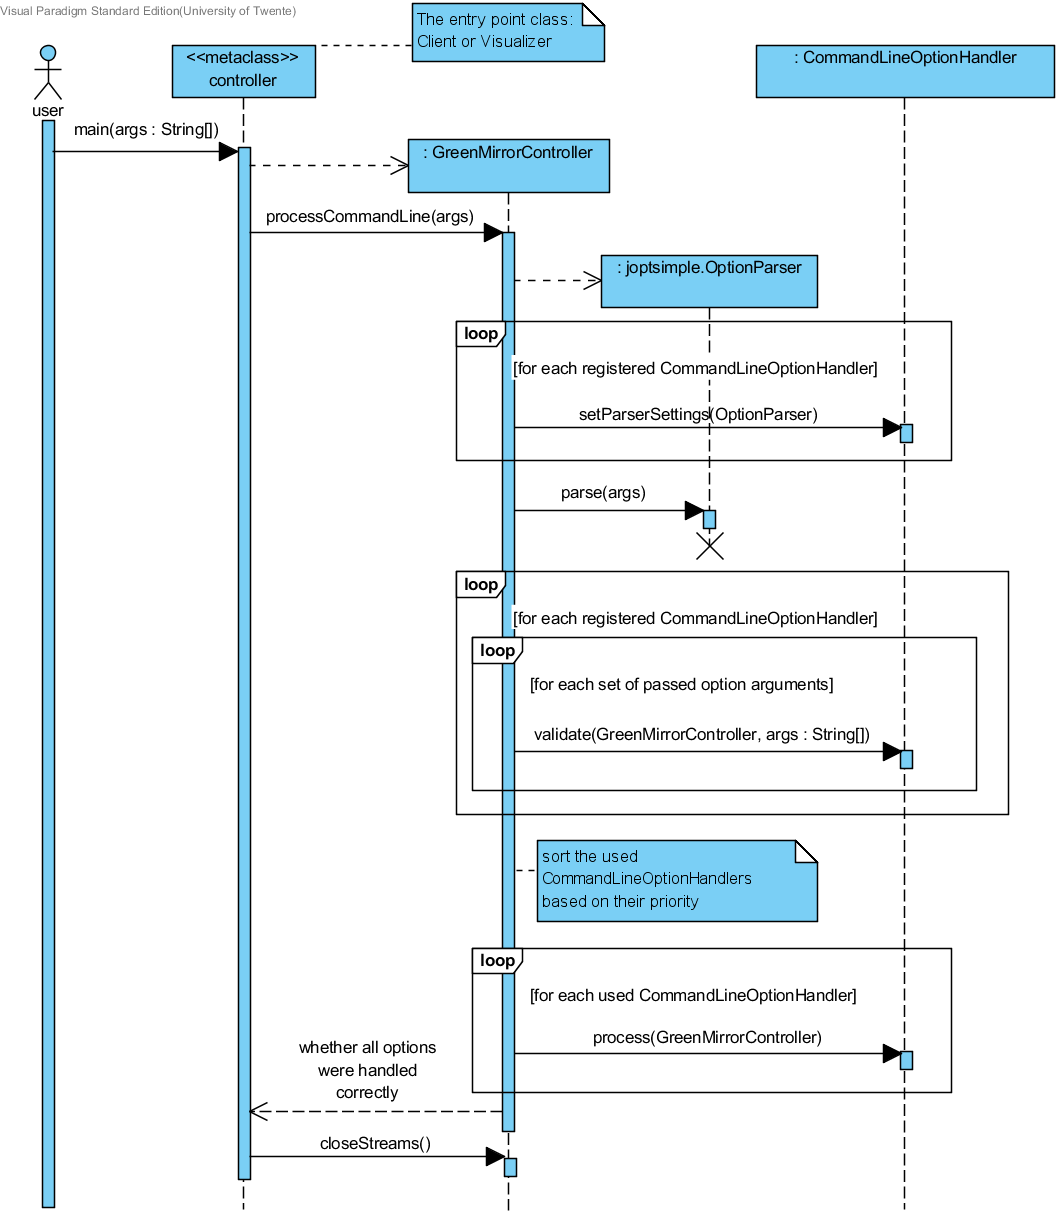
\includegraphics[width=0.96\textwidth]{diagrams/SD_generalstartup}
  }
  \caption{Simplified sequence diagram of the general start-up. There is a slight difference on the server side: if the options are all handled correctly, the controller doesn't close the streams, but starts listening for incoming connections.}
  \label{fig:sd_generalstartup}
\end{figure}

\begin{figure}[ht]
  \centering
  \makebox[\textwidth][c]{
  	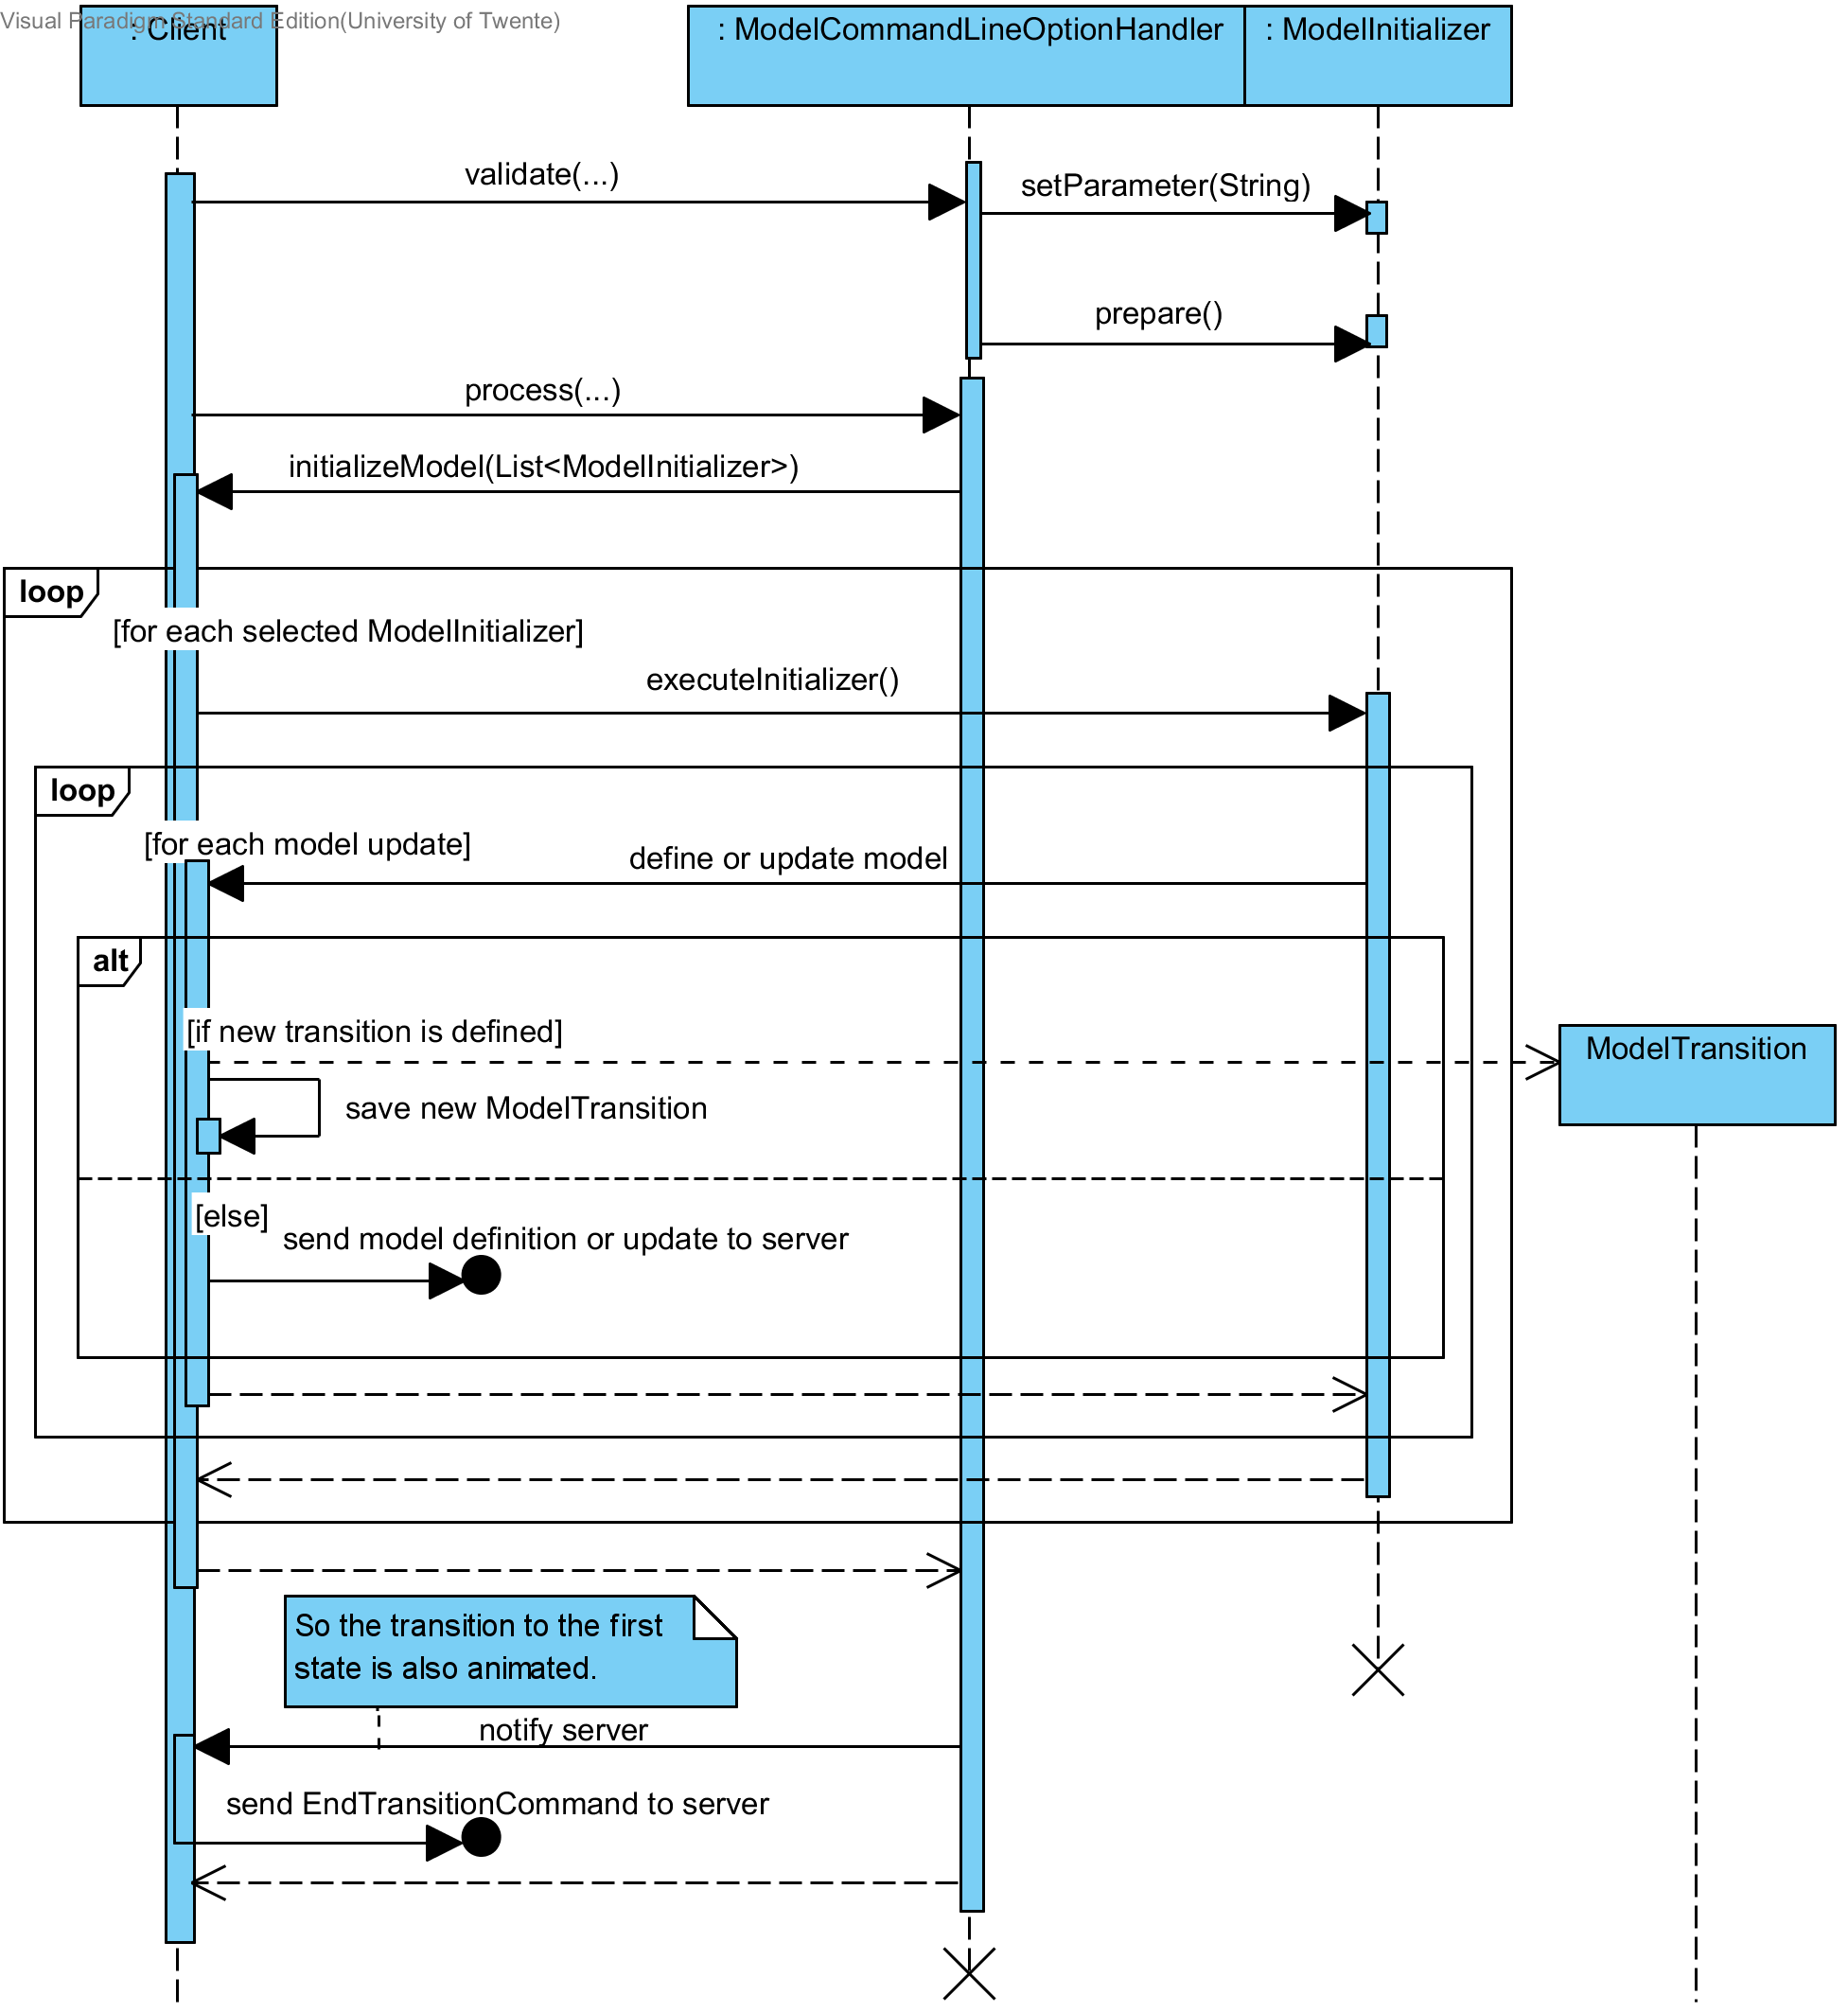
\includegraphics[width=1.1\textwidth]{diagrams/SD_client_model}
  }
  \caption{Simplified sequence diagram of the handling of the \lstinline{--model} command line option}
  \label{fig:sd_client_model}
\end{figure}

\begin{figure}[ht]
  \centering
  \makebox[\textwidth][c]{
  	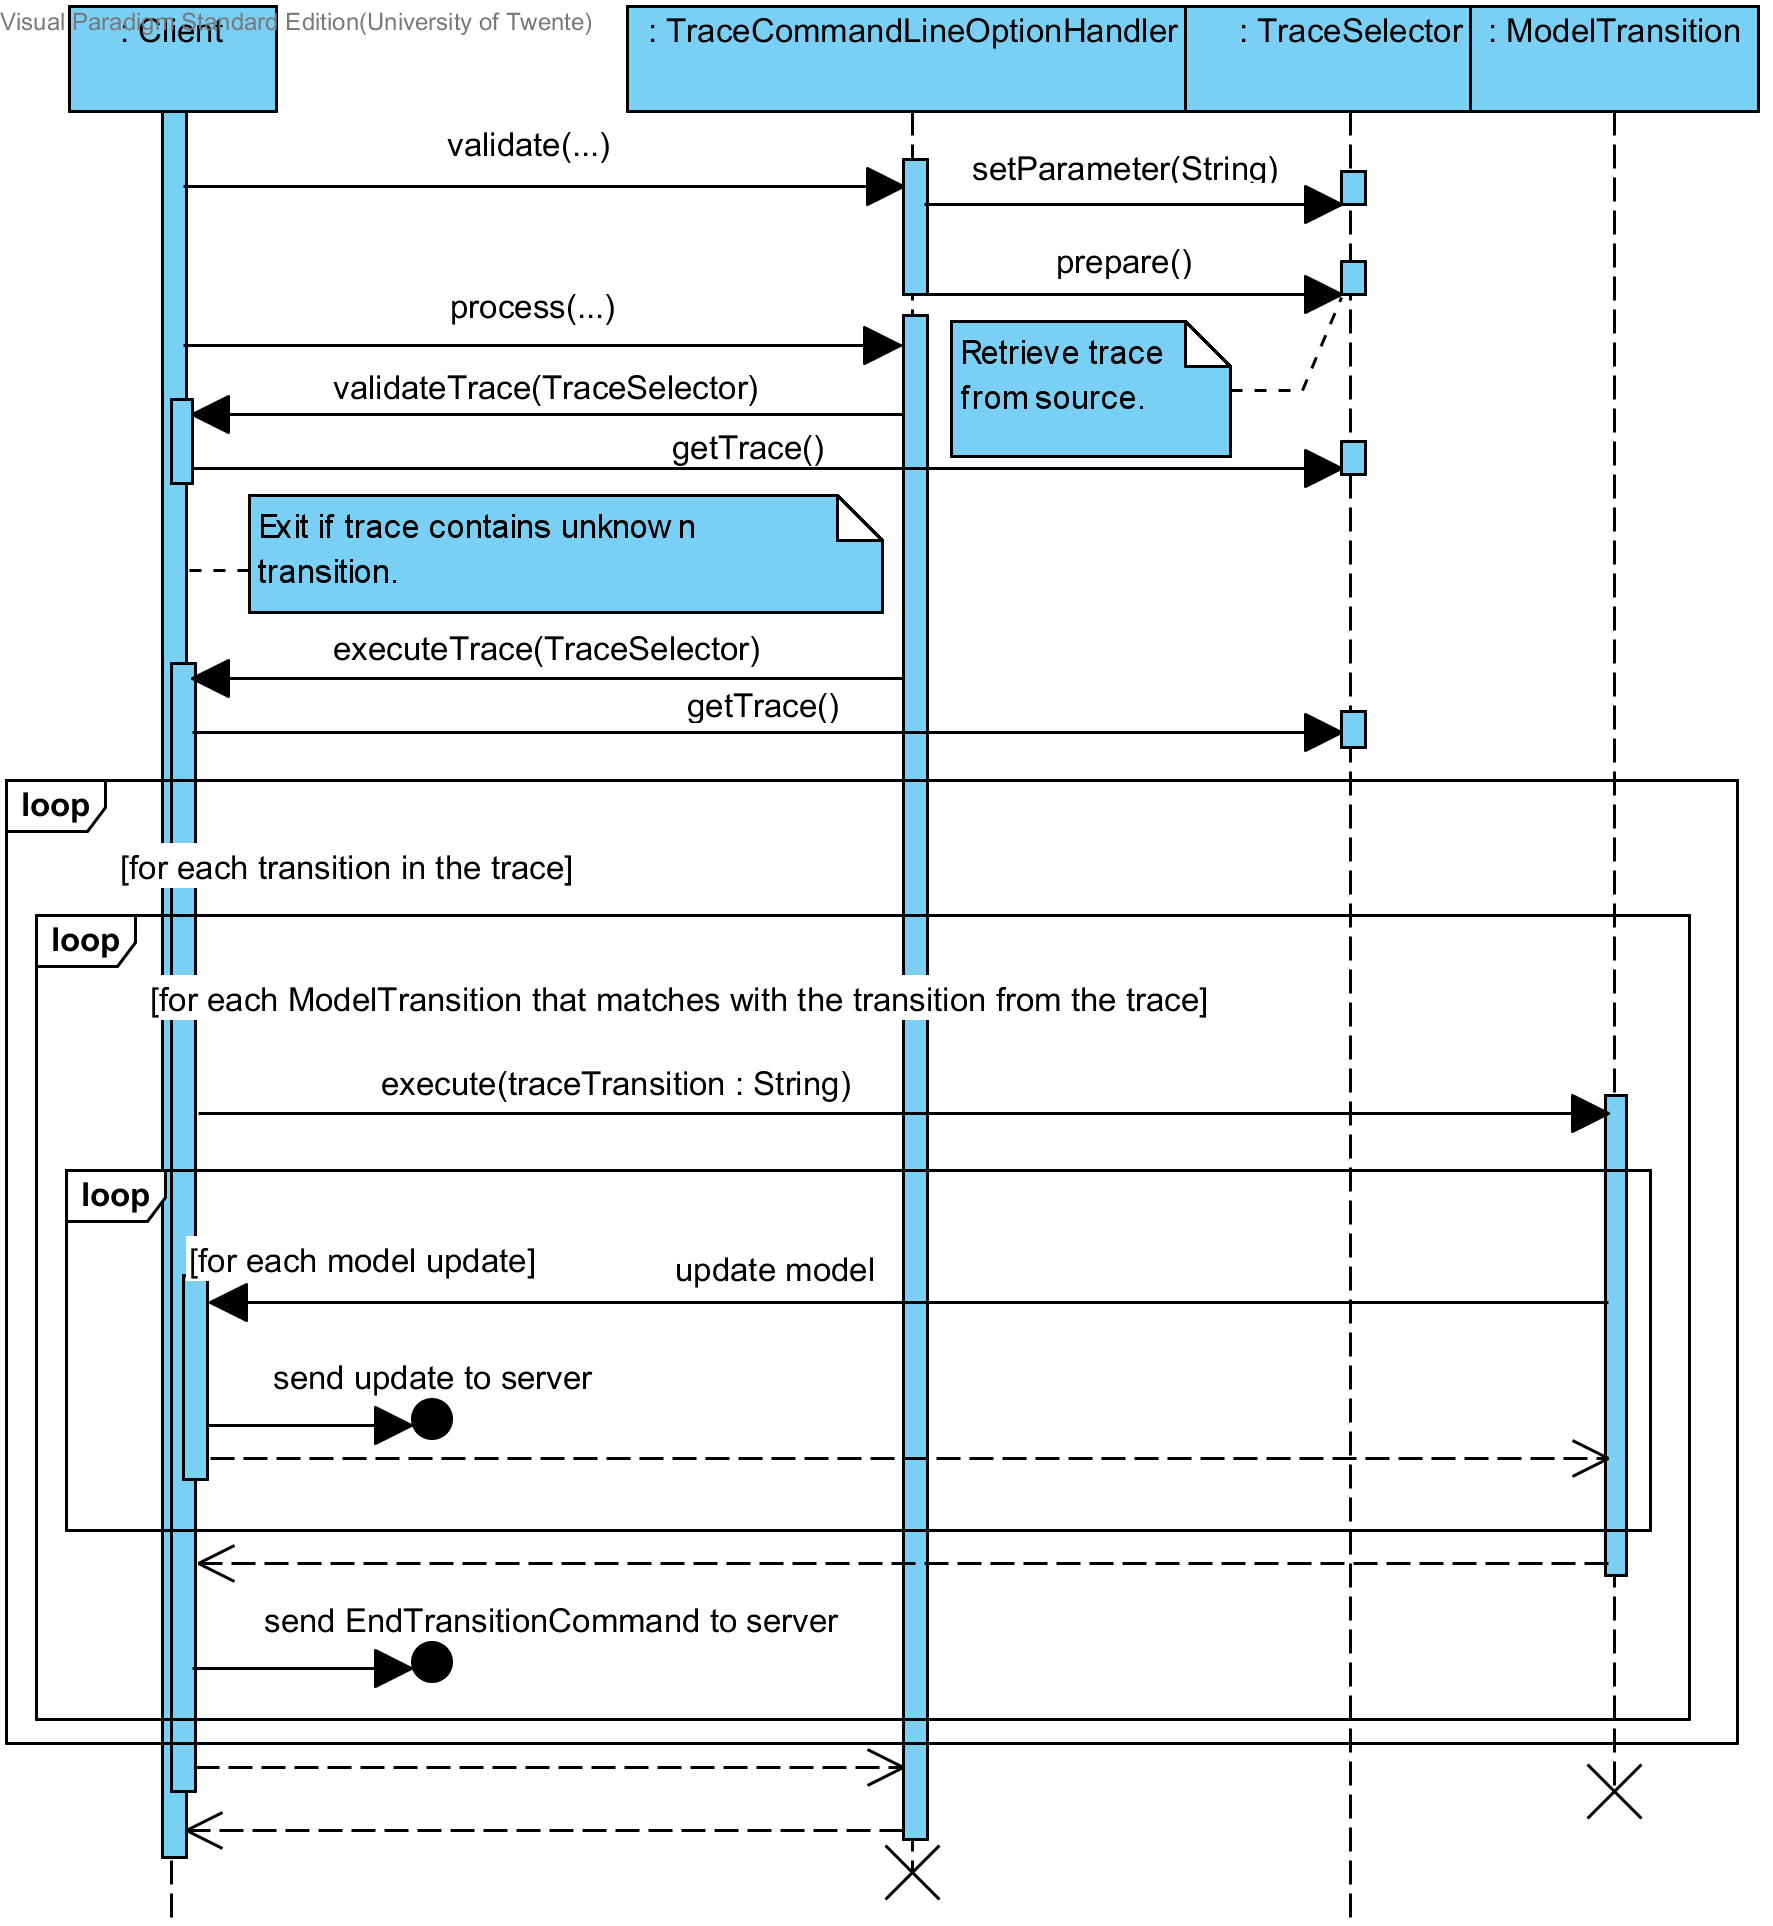
\includegraphics[width=1.1\textwidth]{diagrams/SD_client_trace}
  }
  \caption{Simplified sequence diagram of the handling of the \lstinline{--trace} command line option}
  \label{fig:sd_client_trace}
\end{figure}

\begin{figure}[ht]
  \centering
  \makebox[\textwidth][c]{
  	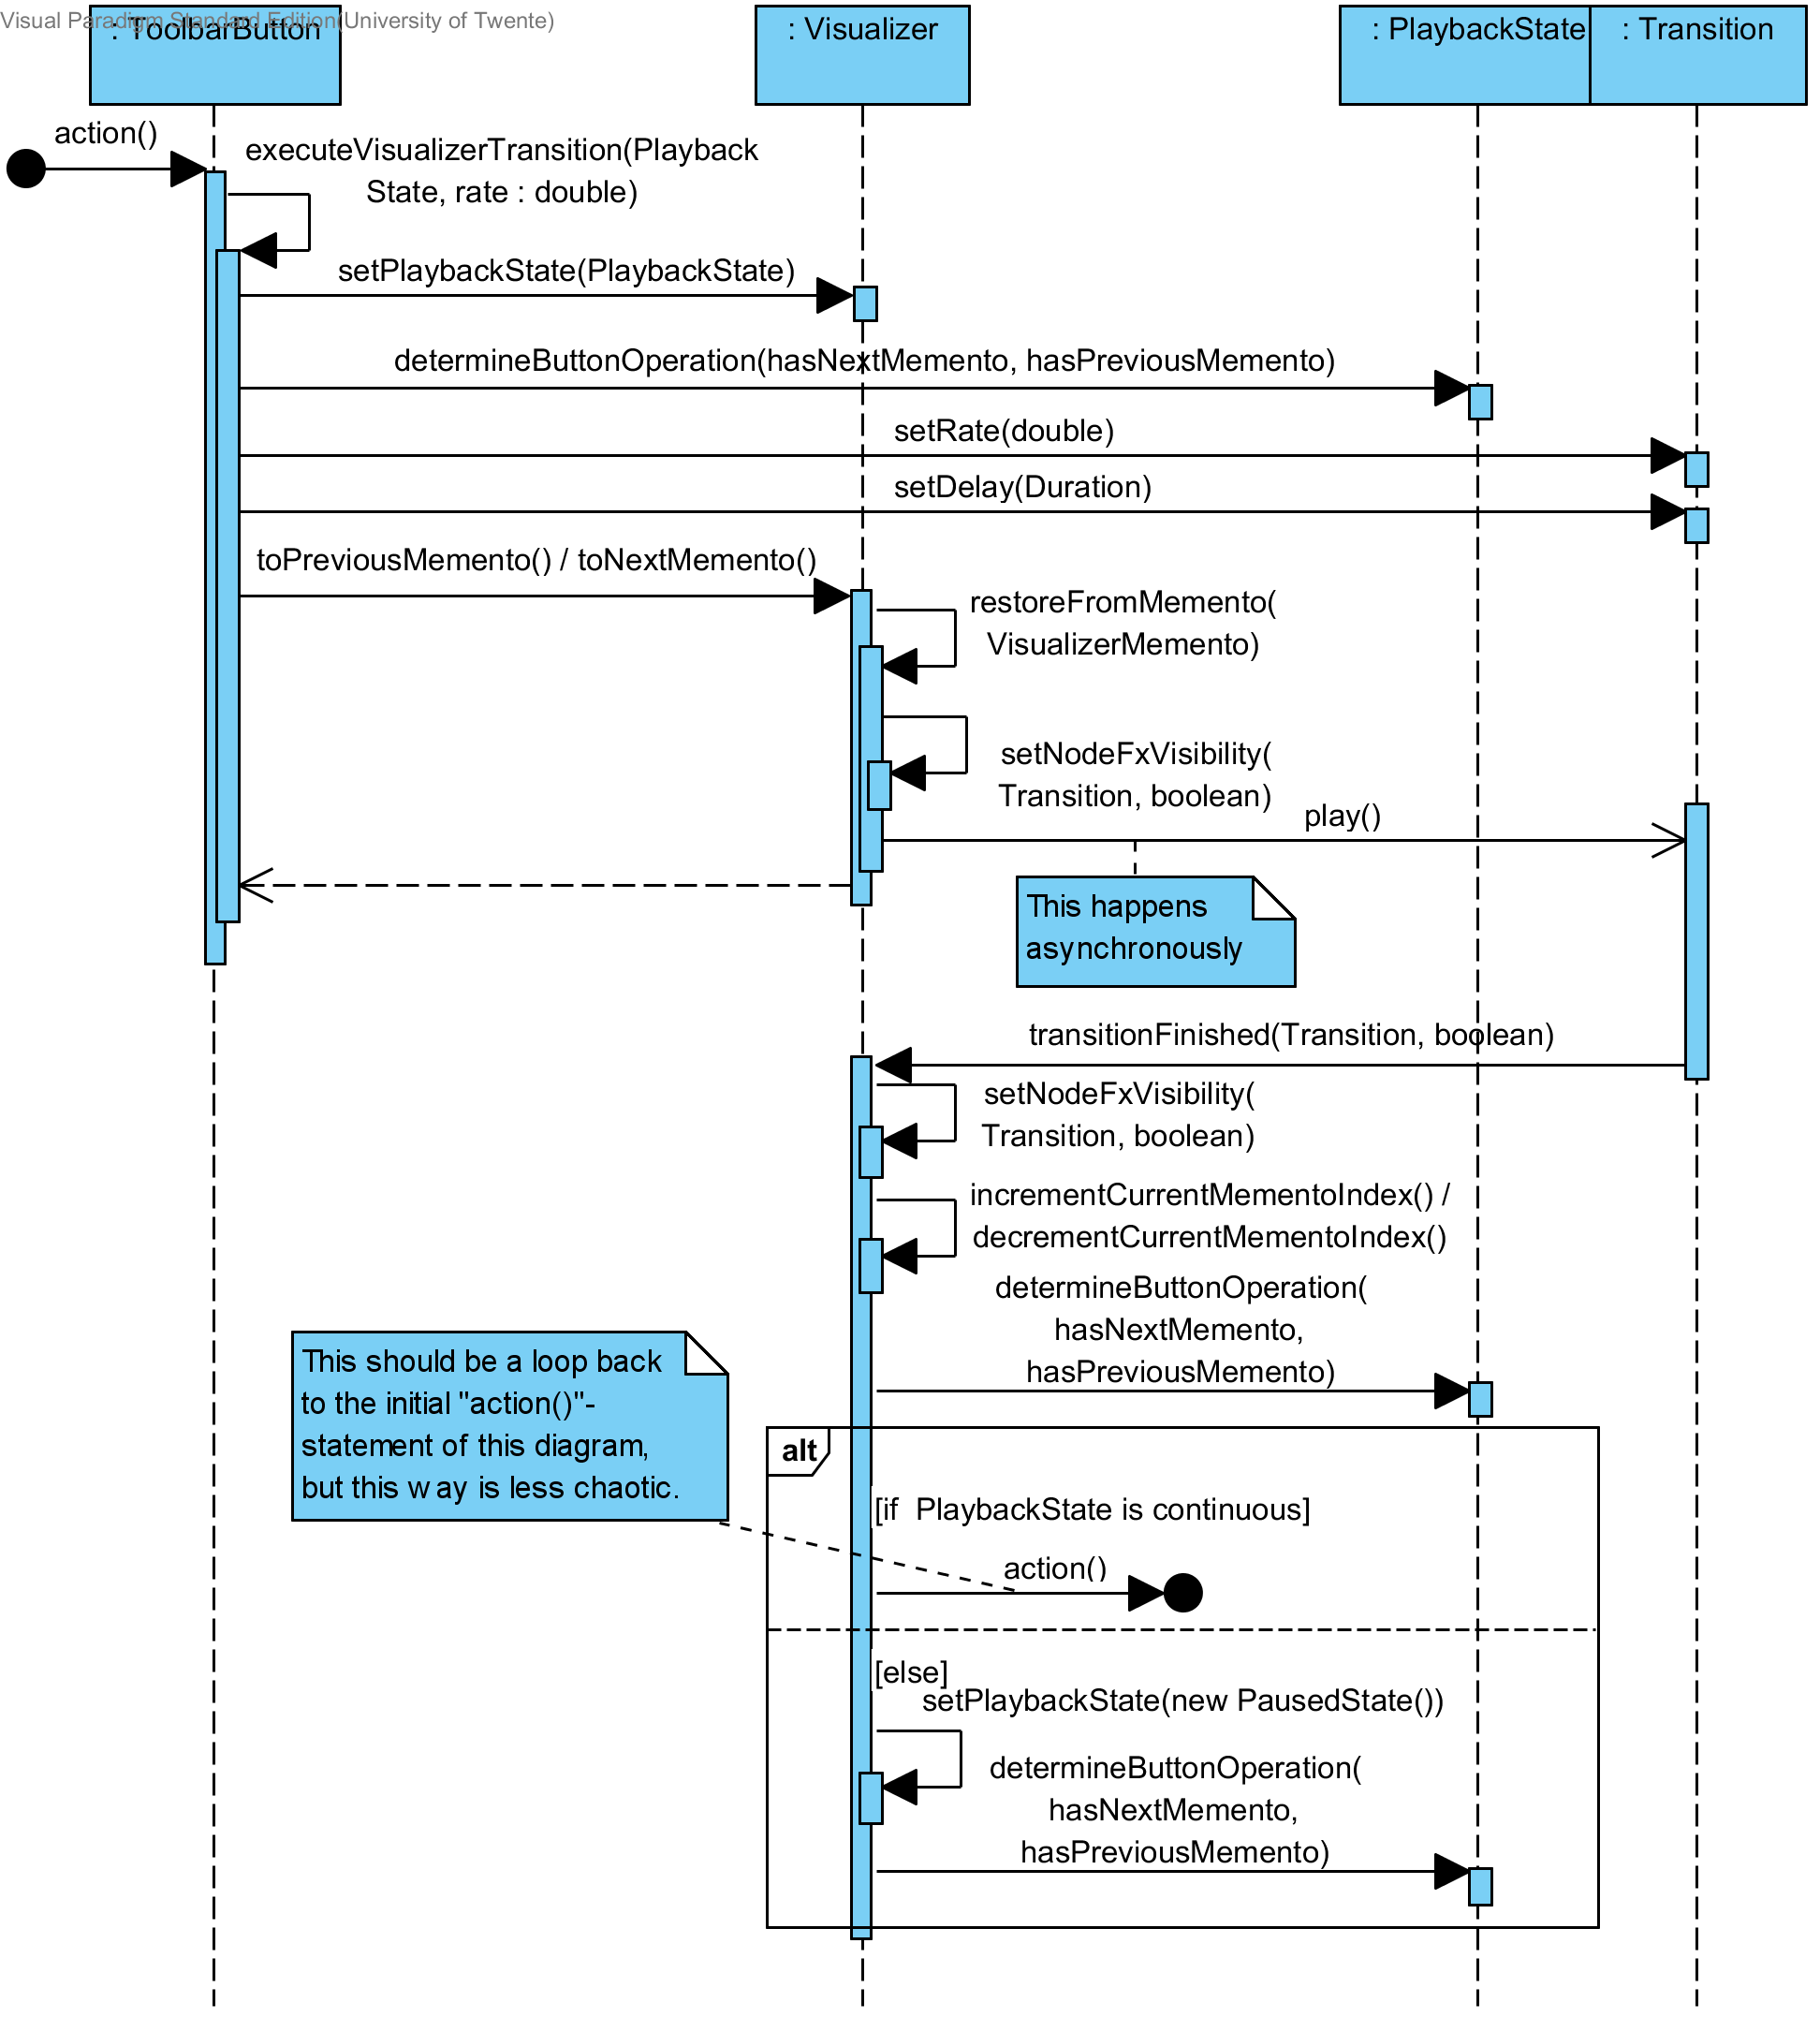
\includegraphics[width=1.1\textwidth]{diagrams/SD_server_userinteraction}
  }
  \caption{Simplified sequence diagram of user interaction with any one of the toolbar buttons (but not with the pause button)}
  \label{fig:sd_server_userinteraction}
\end{figure}


\begin{comment}
Dining philosophers: Dijkstra, E.W. (1968). Cooperating sequential processes. In F. Genuys (ed.) Programming Languages, 43-112. New York: Academic Press.
\end{comment}

\end{document}